\documentclass[aps,pre,preprint]{revtex4-1}
% \documentclass[aps,pre,twocolumn]{revtex4-1}
% \documentclass[aps,jcp,groupedaddress,twocolumn,unsortedaddress]{revtex4}

\usepackage{amsmath}
\usepackage{amssymb}
\usepackage[dvips]{graphicx}
\usepackage{color}
\usepackage{tabularx}

\makeatletter
\makeatother

\newcommand{\recheck}[1]{{\color{red} #1}}
\renewcommand{\v}[1]{\textbf{\textit{#1}}}
\renewcommand{\d}[1]{\textsf{#1}}


\begin{document}

\title{The Error Estimate of Force Calculation in the Inhomogeneous Molecular Systems}
\author{Han Wang}
\affiliation{LMAM and School of Mathematical
  Sciences, Peking University}
\author{Pingwen Zhang}
% \email{pzhang@pku.edu.cn}
\affiliation{LMAM and School of Mathematical
  Sciences, Peking University}

\begin{abstract}
\end{abstract}

\maketitle

\section{Introduction}
Non-bonded short-range interaction is encountered in nearly every
molecular simulation.  A naive idea to calculate short-range
interactions is to explicitly calculate all pairwise
interactions. This results in a computational cost scaling $\mathcal
O(N^2)$ per time step, which rapidly becomes inefficient as the number
of particles $N$ grows large. A better way is to introduce a cut-off
radius, outside of which all pairwise interactions are simply
neglected. In combination with the cell list and the neighbor list
algorithms \cite{frenkel02b}, the total computational cost of the
short-range interactions can be reduced to an acceptable level of
$\mathcal O(N)$.  The cut-off radius neglect all pairwise interactions
outside the cut-off radius, so it introduces error in the interaction
calculation. The cut-offed system could be viewed as approximation of
the original system, therefore, it is very important to test the
convergence of the properties under study with respect to the cut-off
radius before deriving conclusions on the origianl system.

Fortunately,
in most homogeneous systems, a satisfactory convergence can be
achieved even with a very small cut-off value, for example,
$2.5\sigma$.  Moreover, it is possible to correct the systematic error
of the potential energy, the pressure and the free energy by applying
the standard long range correction (LRC)~\cite{allen87a}, which
assumes the uniformity outside the cut-off radius and integrates the
contribution of the mentioned properties to infinity. 
% The spacial inhomogenety of the system in terms of particle density,
% particle type and change distribution is very common in natrual
% system.

The inhomogeneous systems, in which the density of certain type of
atom changes within the length scale of several molecules, are more
universal in nature. However, the direct molecular simulation of
inhomogeneous systems by the cut-off method will encounter non-trival
difficulties that do not exist in the homogeneous system simulations.
The simulation results are found to converge only at a very large
cut-off radius value~\cite{duque2004some, ismail2007application}, also
denpend on the energy/force continuity at the cut-off and the way of
applying the long-range corrections~\cite{trokhymchuk1999computer,
  guo1997long, mecke1997molecular, janecek2006long, goujon2004monte,
  shen2007comparative}.  Therefore, it is necessary to systemetically
study the precision of the short-range interaction calculation, and to
develop methods screening out the aforementioned cut-off artifect in
the inhomogeneous systems.

% In this paper, we focus on the systems in which
% atoms/particles are interacting via short-range interactions, because
% it is a good starting point of the study of more complex systems, for
% example, the systems with long-range electrostatic interactions.  The
% simulation results in the inhomogeneous systems are found to depend on
% a number of factors of treating the short-range interaction in the
% simulation. For example, the way of calculating the short-range
% interaction (simple cut-off method or Ewald
% summation)~\cite{karasawa1989acceleration, lopez2002thermodynamic,
%   lopez2006liquid, shi2006molecular, ismail2007application}, the
% cut-off radius~\cite{trokhymchuk1999computer, duque2004some,
%   shen2007comparative}, the way of long-range
% correction~\cite{guo1997long, mecke1997molecular, janecek2006long,
%   goujon2004monte} and the size and shape of the simulation
% box~\cite{chen1995area, orea2005oscillatory, biscay2009calculation}.
% It should be noticed that the physical properties are the nature of
% the system, and should NOT depend on the details of the interaction
% calculation.


A promising way to quantitatively analyze the undesirable cut-off
effects is to express these artifacts in terms of the difference
between the cut-offed interaction and the exact interaction, namely
the error. In homogeneous systems, the error analysis of the cut-off
method has been well established, see~\cite{kolafa1992cutoff} for
example. Also the error estimates~\cite{hummer1995numerical,
  kolafa1992cutoff, petersen1995accuracy, deserno1998mue2,
  wang2010optimizing} for long-range Ewald family
methods~\cite{ewald1921die, hockney1988computer, deserno1998mue1,
  darden1993pme, essmann1995spm} have provided a profound
understanding of the accuracy of force calculation, and introduced
parameter tuning algorithms~\cite{limbach06a, wang2010optimizing} that
boost the efficiency of the computation with a good control of the
error. However, in inhomogeneous systems the error study is still
scarce, even for the simplest cut-off method.

In this work, we develop the error estimate of the short-range force
in inhomogeneous systems. We prove that the 
force error is comprised of a homogeneity error and a inhomogeneity
error, regardless the particle-particle correlation outside the
cut-off radius.  In a inhomogeneous system composed by several bulk
regions, an important observation is that the inhomogeneity error can
be more than one order of maganitude larger than the homogeneity
error, and plays a dominant role in the interfacial region. An
adaptive cut-off method is hereby proposed to equally distribute the
error across the simulation region, so that a substantial
computational effort can be saved while the precision of simulation is
preserved. We also proposed a long-range force correction (LFC) method
based on the error estimate to screen out the contribution of the
inhomogeneity error, which can tremendously improve the precision of
simulation without much extra computational load. To show the
effectiveness of the error estimate and the proposed methods, two
systems are tested: the liquid-vapor equilibrium for equilibrium
properties, and the colliding nanoscale clusters for dynamical
properties. Finally, conclusions are given in section
\ref{sec:conclusion}.

% The error estimate of long-range algorithms, for example the Ewald
% family method~\cite{ewald1921die, hockney1988computer,
%   deserno1998mue1, darden1993pme, essmann1995spm} and the fast
% multipole method~\cite{greengard1987fast}, has been well developped in
% the past 20 years ~\cite{hummer1995numerical, kolafa1992cutoff,
%   petersen1995accuracy, deserno1998mue2, wang2010optimizing,
%   dachsel2009error}. 



\section{Theoretical background}
\subsection{Error estimate in a inhomogeneous system}

In this paper, we only consider the single-component system. Because
this assumption simplifies the discussion, and the error estimates for
the single-component system can be straightforwardly extended to the
multi-component system without any difficulty.  Only the
force error is estimated in the present paper, because the
applications are based on molecular dynamics simulation.
% Since the error estimate developed for the one-component system can be
% directly extended to multi-component system without substantial
% difficulty, the discussion in this paper will focus on one-component
% system for symplicity. 
Suppose the system is composed by $N$ identical particles located at
$\v r_1, \v r_2, \cdots, \v r_N$ with periodic boundary condition.
These particles are interacting via a short-range pairwise interaction
$u(\v r)$ with a cut-off radius $r_c > 0$. The corresponding force is
denoted by $\v f(\v r)$. 
% An infinite cut-off radius will lead to
% a precise calculation of interaction, but it is impractical.
% The error of computing interaction is mainly introduced by a finit
% value of the cut-off radius.
The force error mainly stems from the neglected interaction outside
the cut-off radius, so it is convenient to consider the complementary
of the cut-offed force that is defined by
\begin{align}
  \v f^c(\v r) =
  \left\{
  \begin{array}{ll}
    0, & \vert\v r\vert\leq r_c; \\
    \v f(\v r), & \vert\v r\vert > r_c.
  \end{array}
  \right.
\end{align}
We measure the force error at an arbitary position in the system,
saying $\v r$, by adding a testing particle to that position.  We
assume all particles in the system exert forces on the testng
particle, whereas the testing particle do NOT exert any force on the
system.  The exact force and the computed force (or cut-offed force)
exerted by the system on the testing particle are denoted by ${\v
  F}(\v r)$ and $\tilde{\v F}(\v r)$, respectively.  The difference
between them, namely the \emph{error force}, is denoted by $\Delta\v
F(\v r) = \v F(\v r) - \tilde{\v F}(\v r)$, which can be expressed by
\begin{align}
  \Delta\v F(\v r) = \sum_{\v n}\sum_{j}\, \v f^c(\v r - \v r_j + \v n).
\end{align}
Where $\v n$ is the box vector, so the summation over $\v n$ indicates
that all periodic images of the system are considered. In a
homogeneous system, the surounding of any particle is isotropic, so
the \emph{mean error force} vanishes: $\langle\Delta\v F(\v r)\rangle
= 0$. In contrast, the mean error force is not necessarily zero in a
inhomogeneous system:
\begin{align} \label{eqn:tmp3} %\nonumber
  \langle\Delta\v F(\v r)\rangle
  &=
  \big\langle
  \sum_{\v n}\sum_{j}\, \v f^c(\v r - \v r_j + \v n)
  \big\rangle 
  =
  \int_{\mathbb R^3}\v f^c(\v r - \v r')\rho(\v r')\,\d d\v r',
\end{align}
where $\rho(\v r)$ denotes the particle number density at the position
$\v r$, and is periodically extended to $\mathbb R^3$. And notice the
error force implicitly depends on the cut-off radius used for the
interaction calculation.

The widely accepted definition of the force error is the \emph{root
  mean square} (RMS) \emph{error}, which is the square root of the second
moment of the error force $\mathcal E(\v r) =
\sqrt{\langle\vert\Delta\v F(\v r)\vert^2\rangle}$. It can be
calculate by
\begin{align} \nonumber
  \langle\vert\Delta\v F(\v r)\vert^2\rangle
  =\,&
  \big\langle\sum_{j,k}\v f^c(\v r - \v r_j)\cdot\v f^c(\v r - \v r_k)\big\rangle \\ \nonumber
  =\,&
  \big\langle\sum_j\vert\v f^c(\v r - \v r_j)\vert^2\big\rangle +
  \big\langle\sum_{j\neq k}\v f^c(\v r - \v r_j)\cdot\v f^c(\v r - \v r_k)\big\rangle \\ \nonumber
  =\,&
  \int_{\mathbb R^3}\vert\v f^c(\v r - \v r')\vert^2\rho(\v r')\,\d d\v r'
  + \\\label{eqn:tmp4}
  \,&
  \int_{\mathbb R^3\times\mathbb R^3}\v f^c(\v r - \v r')\cdot\v f^c(\v r - \v r'')\rho(\v r', \v r'')\,\d d\v r'\d d\v r''.
\end{align}
Where  $\rho(\v r', \v r'')$ is the pair density. By using the identity
\begin{align}  \label{eqn:tmp7}
  \rho(\v r', \v r'')
  = \rho(\v r')\rho(\v r'') + C (\v r', \v r''),
\end{align}
where 
\begin{align}
C (\v r', \v r'') = [\,\rho(\v r', \v r'') -  \rho(\v r')\rho(\v r'')\,]
\end{align}
denotes the density correlation between position $\v r'$ and $\v
r''$. Eqn. \eqref{eqn:tmp4} becomes
\begin{align} \nonumber
  \langle\vert\Delta\v F(\v r)\vert^2\rangle
  = &\,
  \int_{\mathbb R^3}\vert\v f^c(\v r - \v r')\vert^2\rho(\v r')\,\d d\v r' \,+ \\\nonumber
  &\,
  \bigg[\int_{\mathbb R^3}\v f^c(\v r - \v r')\rho(\v r')\,\d d\v r'\,\bigg]^2 + \\\nonumber
  &\,
  \int_{\mathbb R^3\times\mathbb R^3}\v f^c(\v r - \v r')\cdot\v f^c(\v r - \v r'')\,C(\v r', \v r'')\,\d d\v r'\d d\v r'' \\\label{eqn:tmp5}
  = &\,
  \mathcal E^2_{\textrm{homo}}(\v r) +
%  \langle\Delta\v F(\v r)\,\rangle^2 +
  \mathcal E^2_{\textrm{inhomo}}(\v r) +
  \mathcal E^2_{\textrm{correlation}}(\v r).
\end{align}
If the system is homogeneous and the particle-particle correlation is
neglected, then only the first term is left on the right hand side of \eqref{eqn:tmp5}, so it
is called the homogeneity error.  This term originates from the
flucuation of the error force $\Delta\v F(\v r)$.  The second term is
called the inhomogeneity error, because it stems from the density
inhomogeneity of the system. It is worth poining out that the
inhomogeneity error is the nothing but the maganitude of the mean error force,
namely $\mathcal E_{\textrm{inhomo}}(\v r) = \vert\langle\Delta\v F(\v
r)\,\rangle\vert$.  The last term on right hand side of \eqref{eqn:tmp5} originates from the
correlation between the particles, so it is called the correlation
error.
% The correlation error involves a double integral, which
% implies that calculating this term requires more compuational cost
% than the homogeneity and inhomogeneity errors.
The rest of this paper
assumes the 
correlation error does not dominate in the system, and can be savely
neglected.



\subsection{Fast calculation of the error estimate}\label{sec:tmp1.3}

The naive calculation of the convolutions in the error estimate \eqref{eqn:tmp5} requires
a compuational cost of $\mathcal O(N^2)$. To estimate the force error
on the fly, the compuational cost of the estimate should be reduced to
at least $\mathcal O(N\log N)$.  This is achieved by  using the fast Fourier transform. We
assume the simulation box is uniformly divided in to small bins.  The
positions of these bins are
\begin{align}
  \v r_{i_1, i_2, i_3} & =
  \frac{i_1}{K_1}\v a_1 + 
  \frac{i_2}{K_2}\v a_2 + 
  \frac{i_3}{K_3}\v a_3,\qquad 0\leq i_\alpha< K_\alpha
\end{align}
where $\v a_\alpha$ are box vectors, and $K_\alpha$ is the number of
division on each direction. In the reciprocal space, a corresponding
lattice is set up:
\begin{align}
  \v k_{k_1, k_2, k_3} & =
  k_1\v a_1^\ast +
  k_2\v a_2^\ast +
  k_3\v a_3^\ast, \qquad 0\leq k_\alpha<K_\alpha
\end{align}
where $\v a_\alpha^\ast$ are reciprocal box vectors defined by $\v
a_\alpha\cdot\v a_\beta^\ast = \delta_{\alpha\beta}$.  In each bin the
error and the particles number density are assumed to be constant,
then, a Fourier expansion can be obtained:
\begin{align}\nonumber
  \mathcal E^2_{\textrm{homo}}(\v r_{i_1,i_2,i_3})
  & =
  \frac1V\sum_{k_1=-\infty}^\infty\sum_{k_2=-\infty}^\infty\sum_{k_3=-\infty}^\infty
  [{\mathcal E}^2_{\textrm{homo}}]^{\wedge}(\v k_{k_1,k_2,k_3})
  % e^{2\pi i\v k_{k_1,k_2,k_3}\cdot\v r_{i_1,i_2,i_3}}
  \exp\bigg[
  2\pi i\bigg(
  \frac{k_1i_1}{K_1} + \frac{k_2i_2}{K_2} + \frac{k_3i_3}{K_3}
  \bigg)
  \bigg] \\\label{eqn:tmp13}
  & =
  \frac1V\sum_{k_1=0}^{K_1}\sum_{k_2=0}^{K_2}\sum_{k_3=0}^{K_3}
  \hat{K}_{\textrm{homo}}(\v k'_{k_1,k_2,k_3})\:
  \hat{\rho}(\v k_{k_1,k_2,k_3})
  % e^{2\pi i\v k_{k_1,k_2,k_3}\cdot\v r_{i_1,i_2,i_3}}
  \exp\bigg[
  2\pi i\bigg(
  \frac{k_1i_1}{K_1} + \frac{k_2i_2}{K_2} + \frac{k_3i_3}{K_3}
  \bigg)
  \bigg].
\end{align}
Here we denote the convolution kernel $\vert\v f^c(\v r)\vert^2$ by
$K_{\textrm{homo}}(\v r)$.  The second equation in \eqref{eqn:tmp13}
holds due to the fact: the Fourier transform of the convolution
$K_{\textrm{homo}}\ast\rho$ is equal to the multiplication of Fourier transforms
$\hat{K}_{\textrm{homo}}$ and $\hat\rho$, which are given by
\begin{align}\label{eqn:f-kernel-homo}
  \hat K_{\textrm{homo}}(\v k)
  &=
  \int_{\mathbb R^3}K_{\textrm{homo}}(\v r)e^{-2\pi i\v k\cdot\v r}\,\d d\v r,
\end{align}
and
\begin{align}
  \hat\rho(\v k_{k_1,k_2,k_3})
  & =
  \frac{V}{K_1K_2K_3}
  \sum_{i_1=0}^{K_1}\sum_{i_2=0}^{K_2}\sum_{i_2=0}^{K_2}
  \rho(\v r_{i_1,i_2,i_3})
  \exp\bigg[
  -2\pi i\bigg(
  \frac{k_1i_1}{K_1} + \frac{k_2i_2}{K_2} + \frac{k_3i_3}{K_3}
  \bigg)
  \bigg].
\end{align}
In Eqn. \eqref{eqn:tmp13}, the prime on $\v k_{k_1,k_2,k_3}$ means
that the periodic image $k_\alpha - K_\alpha$ should use instead of
$k_\alpha$ when $k_\alpha \geq K_\alpha/2$.  Most of the short-range
interactions are isotropic, i.e.  $K_{\textrm{homo}}(\v r) =
K_{\textrm{homo}}(r)$, then the three-dimensional integral in
Eqn. \eqref{eqn:f-kernel-homo} can be simplified to a one-dimentional
integral:
\begin{align}\label{eqn:kernel-inte}
  \hat{K}_{\textrm{homo}}(\v k)
  =
  % \int_{\mathbb R^3}K_{\textrm{homo}}(r)e^{-2\pi i\v k\cdot\v r}\d d\v r
  % =
  \int_{r_c}^\infty \frac{2 r}k\, K_{\textrm{homo}}(r) \sin(2\pi kr)\,\d dr,
\end{align}
which can be calculated by numerical
integration from $r_c$ to a large upper bound, saying $R_c$. Perfact
convergence can be achieved by using $R_c = 30\sigma$ throughout the
paper. Since integral \eqref{eqn:kernel-inte} is independent with the
density of the system, it can be calculated for only once and stored
for reference.

Similarly, by \eqref{eqn:tmp3}, the Fourier mode of the the mean error
force is
\begin{align}\label{eqn:tmp17}
  \langle\Delta\v F\rangle^\wedge(\v k) =
  \hat{\v f}^c(\v k)\,
  \hat\rho(\v k),
\end{align}
where the Fourier transform of the complementary force is given by
\begin{align}\label{eqn:tmp18}
  \hat{\v f}^c(\v k) 
  & = 
  2\pi\frac{\v k}k\, i\,
  \bigg\{
  r_c^2\,u(r_c)
  \bigg[\,
  \frac{2\cos(2\pi kr)}{2\pi kr}
  -\frac{2\sin(2\pi kr)}{(2\pi kr)^2}
  \,\bigg] 
  -
  \int_{r_c}^\infty 2r\,u(r)\sin(2\pi kr)\,\d d\v r
  \bigg\}.
\end{align}


\subsection{Adaptive cut-off radius method}

% In Fig. \ref{fig:tmp1}, the testing system containing $N=16000$
% standard Lennard-Jone particles is set up in a tube with periodic
% boundary condition. The liquid droplet (in the middle of the tube) is
% in equilibrium with the surrounding vapor environment. The red line in
% the Fig. \ref{fig:tmp2} denotes the density profile (on direction $x$)
% of this inhomogeneous system. The green square denotes the real RMS
% force error distribution. It is clear that the error form two peaks in
% the interfacial region, which is much higher than the relative
% constant error of the bulk liquid and the bulk vapor. The dashed and
% the dotted blue line are the estimated homogeneity and inhomogeneity
% errors, and the solid blue line is the sum. In the bulk region, the
% homogeneity error dominates while in the interfacial region, the
% inhomogeneity error dominates. The esitmated error matches perfactly
% with the real error at the interfacial region, but presents
% overestimation in the bulk regions. The overestimation probably stems
% from the neglection of the correlation error in \eqref{eqn:tmp5}.

A basic observation in a inhomogeneous system is that the RMS force
error is not uniformly distributed. The difference between the maximum
and minimum error can be more than one order of
maganitude,
% in one of the cases we studied,
see Fig. \ref{fig:tmp2}. Traditionally, a very large cut-off radius is
used to reduce the maximum error in the system to reach convergent
simulation results~\cite{ismail2007application}. Therefore, a huge
amount of compuational effort is wasted in the low-error region. The
idea of the adaptive cut-off radius simulation is to use larger
cut-off radius for particles in the high-error region to control the
force error, while to use smaller cut-off radius for particles in the
low-error region to save compuational cost.  The effectiveness of this
method relies on a diliberated cut-off choice for each particle so
that the force error is uniformly distributed across the simulation
region.  Unfortunately, the compuational expense of a naive
implementation of this method is at least $\mathcal O(N^2\log N)$.
Becasue to determine the cut-off radius, we should estimate the RMS
force error at least once for each particle, and the computational
cost of each force error estimate is $\mathcal O(N \log N)$.


% Since inhomogeneity error dominate the
% force error of the system, such a big cutoff radius is a waste in the
% bulk liquid and vapor regions. One possible way is to use adapt
% cut-off radius according to the error distribution, so that larger
% cut-off radii are used in the interfacial region while smaller cut-off
% radii are used in the bulk regions.  More precisely, the aim of the
% adaptive cut-off method is to equivalently distributed the force error
% over the simulation region.

To make the adaptive cut-off method feasible, we assume
\begin{enumerate}
\item The space is uniformly divided in to small bins, the size of which is the
  same as those mentioned in the section \ref{sec:tmp1.3}.  The
  particles falling in the same bin are assigned by the same cut-off
  radius. In other words, the cut-off radius is chosen for each bin
  rather than for each particles.
  % The cut-off
  % radius is assumed to be constant within a bin, no matter the
  % position of the partile.
\item The cut-off radius can only be chosen from a discrete series of
  monotonically increasing values between a maximum 
  $r_c^{\textrm{max}}$ and a minimum 
  $r_c^{\textrm{min}}$: $\{\,r_c^{\textrm{min}} = r_c^0 < r_c^1 <
  \cdots < r_c^{M-1} <r_c^M = r_c^{\textrm{max}}\}$.  We call it the
  \emph{candidate set} of the cut-off radius.  For convenience but not
  necessarily, the cut-off radii in the candidate set is uniformly increasing, i.e.
  \begin{align}
    r_c^m = r_c^0 + r_c^{\textrm{step}} m, \quad 0 \leq m \leq M.
  \end{align}
  For example, a possible candidate set is $\{2.5\,\sigma,\
  3.0\,\sigma,\ 3.5\,\sigma,\ 4.0\,\sigma,\ \cdots,\ 10.0\,\sigma\}$,
  with $r_c^{\textrm{max}} = 10.0\sigma$, $r_c^{\textrm{min}} =
  2.5\sigma$ and $r_c^{\textrm{step}} = 0.5 \sigma$.
\end{enumerate}
For each cut-off radius in the candidate set, the force error
$\mathcal E(\v r)$ is calculated by estimate
\eqref{eqn:tmp5}. Notice the error is calculated by the
fast algorithm described in section \ref{sec:tmp1.3}, so it is
defined on the bins.  For a predetermined error control level
$\mathcal E_{\textrm{C}}$, a satisfactory cut-off radius for a bin is
choosen such that it is the smallest one satisfying the precision
constrain $\mathcal E(\v r_{i_1,i_2,i_3}) \leq \mathcal
E_{\textrm{C}}$. The computational cost of this algorithm is $\mathcal
O(MN\log N)$.  The idea of this algorithm is based on the observation
that the cut-off radius may not be calculated at a very high
precision, a slightly (at most $r_c^{\textrm{step}}$) larger
cut-off radius will not waste too much computational cost.  Due to the
thermodynamic flucuation of the system density, the resulting cut-off
distribution $r_c(\v r_{i_1,i_2,i_3})$ (as a function of bin
position) needs to be refined for several times by the following scheme:
\begin{align}\label{eqn:rc-refine}
  r^{(1)}_c(\v r_{i_1,i_2,i_3}) = \max_{j_\alpha\in I}\,r_c(\v r_{i_1+j_1,i_2+j_2,i_3+j_3}),
  \quad I = \{-1, 0, 1\},
\end{align}
so that the fluctuating large-error regions are savely covered by bins
with large cut-off radius.

% This
% means the force error is a combination of a homogeneous contribution,
% a inhomogeneous contribution and a correlational contribution. The
% inhomogeneous force can be applied as a correction to the error:
% \begin{align}\label{eqn:tmp7}
%   \v F_{\textrm{inhomo}} = \int_{\mathbb R^3}\v F^c(\v r - \v r')\rho(\v r')\,\d d\v r'
% \end{align}

\subsection{Long-range Force correction}

In a inhomogeneous system, the inhomogeneity error may play a
dominate role in the simulation, (see examples in section
\ref{sec:tmp2}).  Since the mean error force can be calculated
by~\eqref{eqn:tmp17} on the fly, a simple way to screen out the
inhomogeneity error is to correct the computed force by the mean error
force, namely
\begin{align}\label{eqn:define-fcorr}
  \v F_{\textrm{corr}}(\v r) = \tilde{\v F}(\v r) + \langle\Delta\v F(\v r)\rangle.
\end{align}
In this paper, the mean error force $\langle\Delta\v F(\v r)\rangle$
is also refered as \emph{correction force} in the context of
long-range force correction. This correction works because it takes
into the force contribution outside the cut-off radius. The mean of
the corrected error force vanishes:
\begin{align}\label{eqn:mean-fcorr}
  \langle\Delta\v F_{\textrm{corr}}(\v r)\rangle
   =
  \big\langle\,
  \v F(\v r) - \tilde{\v F}(\v r) - \langle\Delta\v F(\v r)\rangle\,
  \big\rangle = 0.
\end{align}
The mean square error is given by
\begin{align} \nonumber
  \langle\vert\Delta\v F_{\textrm{corr}}(\v r)\vert^2\rangle
  & =
  \big\langle\,
  [\,\v F(\v r) - \tilde{\v F}(\v r) - \langle\Delta\v F(\v r)\rangle\,]^2
  \big\rangle \\\nonumber
  & =
  \big\langle\,
  [\,\Delta\v F(\v r) - \langle\Delta\v F(\v r)\rangle\,]^2
  \big\rangle \\\nonumber
  & =
  \langle\vert\Delta\v F(\v r)\vert^2\rangle -
  \langle\Delta\v F(\v r)\,\rangle^2 \\
  & =
  \mathcal E^2_{\textrm{homo}}(\v r) +
  \mathcal E^2_{\textrm{correlation}}(\v r),
\end{align}
containing no inhomogeneity contribution.  It worth noticing that the mean
square error of the corrected force is nothing but the variance of the
corrected/uncorrected error force: $\langle\vert\Delta\v
F_{\textrm{corr}}(\v r)\vert^2\rangle = \textrm{Var}[\Delta\v
F_{\textrm{corr}}(\v r)] = \textrm{Var}[\Delta\v F(\v r)]$.

The idea of the long-range force correction is very similar to those
proposed by earlier works~\cite{guo1997long, mecke1997molecular,
  janecek2006long, shen2007comparative}. In those works, the density
profile is assumed to be inhomogeneous on only one direction, and the
system is subdivided into slabs perpendicular to that direction to
calculate the energy/force correction. The advantange of the our force
correction is that it has no geometric restriction on the density
profile of the system, so can be used in a wider range of
inhomogeneous simulations.

% \textrm{Var}[\Delta\v F_{\textrm{corr}}(\v r)] = 

% This means if we correct the computed force by the mean of the error
% force, namely applying to each particle $\tilde{\v F}^c(\v r) =
% \tilde{\v F}(\v r) - \langle\Delta\v F(\v r)\rangle$ instead of
% $\tilde{\v F}(\v r)$. 



\subsection{Long-range pressure correction}
% By the cut-off method, the system lost the pressure contribution from
% the particles outside the cut-off radius.  In the homogeneous systems,
% the distribution of particles is assumed to be uniform outside the
% cut-off radius, and the pressure correction is calculated by
% integrating the virial from the cut-off to infinity.

% In the inhomogeneous systems, the previous idea does not
% work. Instead, the pressure correction of the system are:

The pressure contribution outside the cut-off radius can be expressed
by:
\begin{align}
  \v P^c &= \frac1{V} \bigg\langle \sum_{i\neq j}\,\frac12\, (\v r_i - \v r_j) \otimes \v f^c(\v r_i - \v r_j) \bigg\rangle
\end{align}
For simplicity, we denote $\frac{1}{2V}\v r\otimes\v f^c$ by $\v
K_{\textrm{P}}$, therefore,
% For simplicity, let us consider the general form the the corrections:
% \begin{align}
%   Q = \bigg\langle \sum_{i\neq j} K(\v r_i - \v r_j) \bigg\rangle
% \end{align}
% For the pressure correction, $K$ is replaced by $\frac{1}{2V}\v
% r\otimes\v f^c$.  By using \eqref{eqn:tmp7}, we have
\begin{align}\nonumber
  \v P^c
  &= \bigg\langle \sum_{i\neq j} \v K_{\textrm{P}}(\v r_i - \v r_j) \bigg\rangle\\\nonumber
  & = \int_{\mathbb R^3\times\mathbb R^3}
  \v K_{\textrm{P}}(\v r' - \v r'') \rho(\v r', \v r'') \d d\v r'\d d\v r'' \\\nonumber
  & = \int_{\mathbb R^3\times\mathbb R^3}
  \v K_{\textrm{P}}(\v r' - \v r'')
  \big[
  \rho(\v r') \rho(\v r'') + C(\v r', \v r'')
  \big]
  \d d\v r'\d d\v r''
\end{align}
Assuming the correlation term $C(\v r', \v r'')$ vanishes, then
\begin{align} \nonumber
  \v P^c
  & = \int_{\mathbb R^3\times\mathbb R^3} \v K_{\textrm{P}}(\v r' - \v r'')
  \rho(\v r') \rho(\v r'') 
  \d d\v r'\d d\v r'' \\
  & = \int_{\mathbb R^3}
  \Big[
  \int_{\mathbb R^3} \v K_{\textrm{P}}(\v r' - \v r'') \rho(\v r'')\,\d d\v r''
  \Big]
  \rho(\v r')\,\d d\v r'
\end{align}
The Fourier transform of the convolution $\int \v K_{\textrm{P}}(\v r'
- \v r'') \rho(\v r'')\,\d d\v r''$ is identical to the product $\hat
{\v K}_{\textrm{P}}(\v k)\,\hat \rho(\v k)$.
Assuming the isotropicity of the short-range interaction,
the $\alpha\beta$ component of $\v K_{\textrm{P}}$ can be written as
\begin{align}
  \{\v K_{\textrm{P}}\}_{\alpha\beta}
  = \frac1{2V}\{\v r\otimes\v f^c\}_{\alpha\beta}
  = \frac1{2V} r_\alpha r_\beta \,G^c(r)
  \qquad \alpha, \beta = 1, 2, 3,
\end{align}
where $G^c(r) = [u^c(r)]'/r$ is isotropic.  We list
here without proving the Fourier transform of these terms:
\begin{align}
  [\,r_1r_1\,G^c(r)\,]^{\wedge} 
  =\,& 
  \int_{r_c}^\infty \d dr\, r^4 G(r)\,
  \pi \sqrt{ \frac1{kr} }\,
  \Big[\,
  \frac23\,J_{\frac12}(2\pi kr) -
  \big(\,
  \frac13 -
  \cos^2\Phi +
  \sin^2\Phi\cos2\Theta
  \big)\, J_{\frac52}(2\pi kr)
  \,\Big] \\
  [\,r_2 r_2\,G^c(r)\,]^{\wedge} 
  =\,& 
  \int_{r_c}^\infty \d dr\, r^4 G(r)\,
  \pi \sqrt{ \frac1{kr} }\,
  \Big[\,
  \frac23\,J_{\frac12}(2\pi kr) -
  \big(\,
  \frac13 -
  \cos^2\Phi -
  \sin^2\Phi\cos2\Theta
  \big)\, J_{\frac52}(2\pi kr)
  \,\Big]   \\
  [\,r_3 r_3\,G^c(r)\,]^{\wedge} 
  =\,& 
  \int_{r_c}^\infty \d dr\: \,r^4 G(r)\,\pi\,
  \sqrt{ \frac1{kr} }\,
  \Big[\,
  \frac23 J_{\frac12}(2\pi kr) +
  \big(\,
  \frac23 - 2\cos^2\Phi
  \big)
  J_{\frac52}(2\pi kr)
  \,\Big]\\
  [\,r_1 r_2\,G^c(r)\,]^{\wedge} 
  =\,& -
  \int_{r_c}^\infty
  \d dr\,
  r^4G(r)\,\pi\,
  \sqrt{\frac1{kr}}\:
  \sin^2\Phi\sin 2\Theta\,J_{\frac52}(2\pi kr)\\
  [\,r_1 r_3\,G^c(r)\,]^{\wedge} 
  =\,& -
  \int_{r_c}^\infty
  \d dr\,
  r^4G(r)\,\pi\,
  \sqrt{\frac1{kr}}\:
  \sin2\Phi\cos\Theta\,J_{\frac52}(2\pi kr)\\
  [\,r_2 r_3\,G^c(r)\,]^{\wedge} 
  =\,& -
  \int_{r_c}^\infty
  \d dr\,
  r^4G(r)\,\pi\,
  \sqrt{\frac1{kr}}\:
  \sin2\Phi\sin\Theta\,J_{\frac52}(2\pi kr)
\end{align}
Where $(k, \Phi, \Theta)$ are the spherical coordinates of reciprocal
variable $\v k$, and $J_\nu(x)$ is the Bessel function of the first
kind.



\section{Testing simulations and discussions}\label{sec:tmp2}

\subsection{Liquid-vapor equilibrium}\label{sec:tmp2.1}

The direct simulation of the liquid-vapor equilibrium is a very
typical inhomogeneous system, which is widely used to study the phase
coexistence properties, for example, the equilibrium liquid/vapor
density, and the surface tension. The system studied in the present
paper contains 16,000 identical standard Lennard-Jones particles that are
saperated into liquid phase in the center of the box and vapor phase
surrounded, see Fig.~\ref{fig:tmp1}.  The conventional dimensionless
unit system is employed: the unit of length, energy, mass and time are
denoted by $\epsilon$, $\sigma$, $m$ and $\tau$ ($\tau =
\sigma\sqrt{m/\varepsilon}$), respectively.  All quantities are
written in the unitless form by adding the superscript ``$\ast$''.
For example, $r^\ast = r / \sigma$, $T^\ast = k_BT / \epsilon$,
$P^\ast = P\cdot \sigma^3 / \epsilon$ and $\mathcal E^\ast = \mathcal
E\cdot\sigma/\varepsilon$.  The MD time step {is} $\Delta t^\ast =
0.005$. The simulations last for $3\times 10^6$ time steps. The first
$1\times 10^6$ steps are discarded. The quantities of interest are
sampled every 100 time steps. The blocking average
method~\cite{flyvbjerg1989error} is applied to estimate the
statistical uncertainty of the autocorrelated data with 95\%
confidence level. The NVT ensemble is generated by the Nos\`e-Hoover
thermostat~\cite{nose1984molecular, hoover1985canonical}.  The size of
the simulation box is $L_x^\ast \times L_y^\ast \times L_z^\ast =
150\times 21\times 21$, which permits a maximum cut-off radius of
$r_c^\ast = 10$, and eliminates the finite size effect reported in
literatures \cite{chen1995area, orea2005oscillatory,
  biscay2009calculation}.
The system is divided into bins of size $1\times1\times1$ to perform the fast error
estimate method described in section \label{sec:tmp1.3}.
In all simulations, the maximum cut-off
radius considered is $10$, but the reference results for comparison
are obtained by simulations carried out in a 24,000 particles system
with simulation box $L_x^\ast \times L_y^\ast \times L_z^\ast =
150\times 27\times 27$, and a uniform cut-off radius of $r_c^\ast =
13$.

\begin{figure}
  \centering
  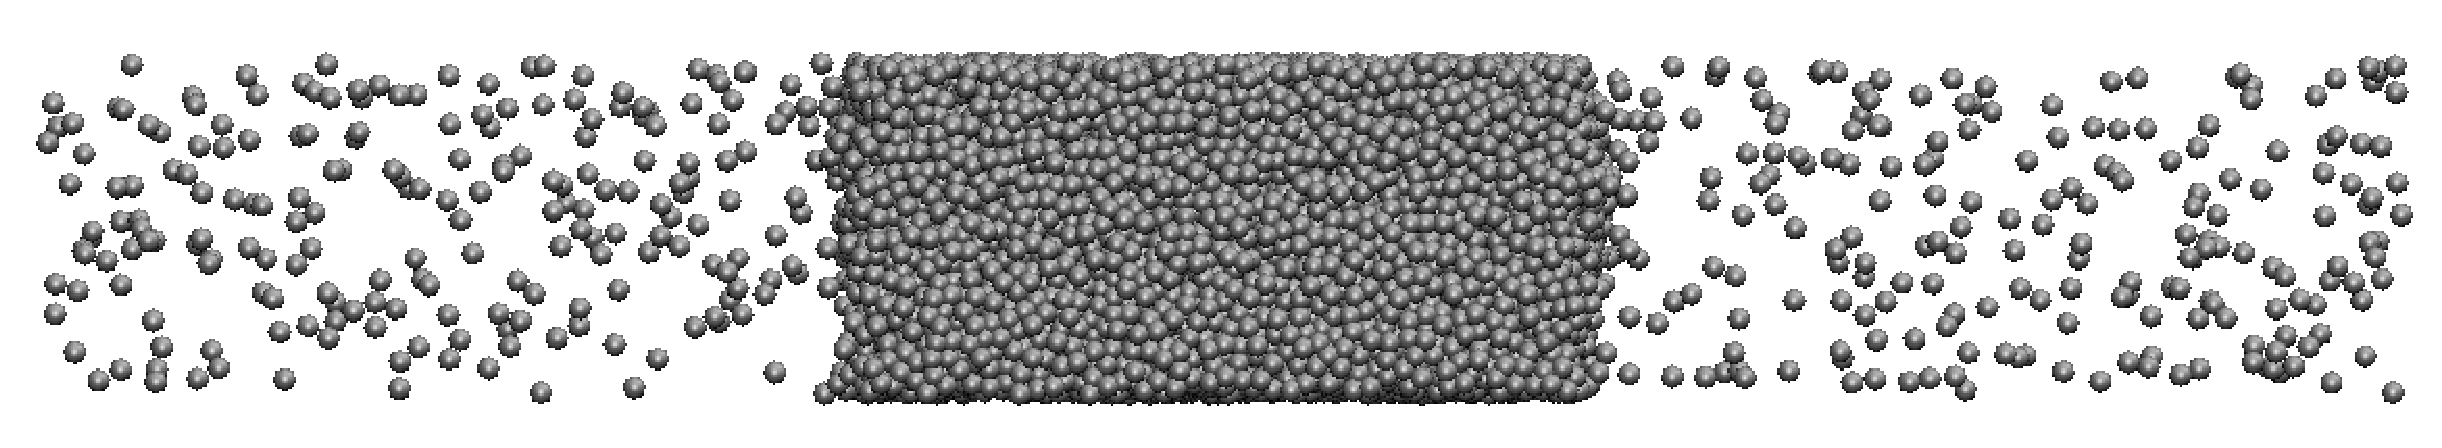
\includegraphics[width=0.9\textwidth]{fig/t0.85-n16000-rc07.5uni/confout.eps}
  \caption{The snapshot of the 16000 Lennard-Jones particle system in
    liquid-vapor equilibrium at $T^\ast=0.85$ with a uniform cut-off
    radius of $r_c^\ast = 7.5$.}
  \label{fig:tmp1}
\end{figure}

Figure \ref{fig:tmp2} presents the real RMS force error (in green
square and log-scaled) in a system using a uniform cut-off raidus of $r_c^\ast =
7.5$. The number density distribution along $x$ direction is shown by
the solid red line for reference.  The error is comparatively constant
at the bulk liquid and gas region. In contrast, two paaks, which are
more than one order of maganitude larger than the force errors in bulk
regions, form at the interfacial region.  The estimated RMS force
error is presented by solid blue line.  The estimate follows the real
error very well at the interfacial region, but slightly over estimate
the error in the bulk regions.  Two components of the force error,
namely the homogeneity error and inhomogeneity error are presented in
Fig. \ref{fig:tmp2} by dashed and dotted blue lines, respectively.  In
the bulk regions, the dashed blue line overlaps with the solid blue
line, that means the homogeneity error dominates.  In the interfacial
region, in the contrary, the inhomogeneity error dominate, because the
dotted blue line overlaps with the solid one.

\begin{figure}
  \centering
  % 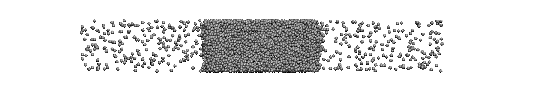
\includegraphics[]{fig/t0.85-n16000-rc07.5uni/confout-02.eps}
  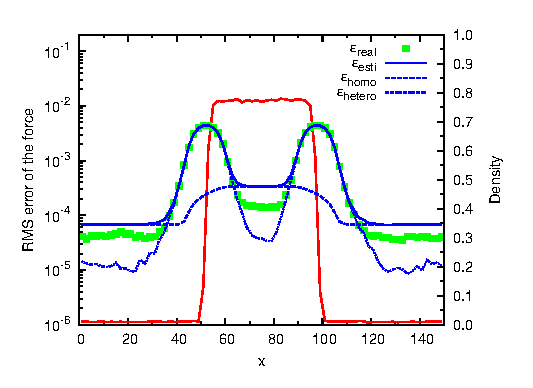
\includegraphics[]{fig/t0.85-n16000-rc07.5uni/error.uniform.eps}
  \caption{The RMS force error distribution of the 16000 Lennard-Jones
    particle system at $T^\ast=0.85$ with a uniform cut-off radius of
    $r_c^\ast = 7.5$. The green squares present the real error. The
    solid blue line is the error estimate by \eqref{eqn:tmp5}. The
    dashed blue line is the homogeneity error contribution, while the
    dotted blue line is the inhomogeneity error contribution. The
    density distribution of the system is presented by red solid line
    for reference.  All properties are properly averaged on the $y$
    and $z$ direction, therefore, the profiles are plotted along the
    $x$ direction.  }
  \label{fig:tmp2}
\end{figure}


% The Fig. \ref{fig:tmp2} inspires us to develop the adaptive cut-off
% method: in the bulk regions, the error is much smaller, therefore, it
% is a waste to use the same cut-off radius as the interfacial
% regions.
As mentioned before, the key idea of the adaptive cut-off simulation
is to use smaller cut-off
radius in the bulk regions, so that the RMS force error is uniformly
distributed over the simulation region. In Fig. \ref{fig:tmp3}, we
present the adapted cut-off radius by a solid red line and all errors
by the same notations as in the Fig. \ref{fig:tmp2}. The control error
$\mathcal E^\ast_{\textrm{C}} = 0.0045$ is the same as the maximum
error in the uniform cut-off simulation with $r_c^\ast=7.5$. The
cut-off distribution is calculated every 20,000 time steps, and is
refined for twice by \eqref{eqn:rc-refine}. In the interfacial
regions, the same cut-off radius as the uniform cut-off simulation,
namely $7.5$, is used.  In the
liquid and vapor regions, the cut-off radii are $4.75$ and $3.5$,
respective, which is notably reduced. Since the computational cost
grows with $\mathcal O(r_c^3)$, the adaptive cut-off saves 75 \% and
90 \% computational cost in the liquid and vapor bulk regions,
respectively.  The error is uniformly distributed, except in the
liquid region where the real error is somewhat lower.
In constrast with the uniform
cut-off case, i.e. Fig. \ref{fig:tmp2}, the error estimate for the
vapor region is very sharp. The similar phenominon is observed in
Ref.~\cite{wang2011}. The same as the uniform cut-off simuation, the
homogeneity error dominates in the bulk regions, while the
inhomogeneity error dominates in the interfacial region.

\begin{figure}
  \centering
  % 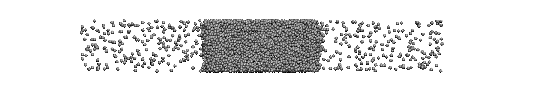
\includegraphics[scale=1]{fig/t0.85-n16000-rc07.5uni/confout-02.eps}
  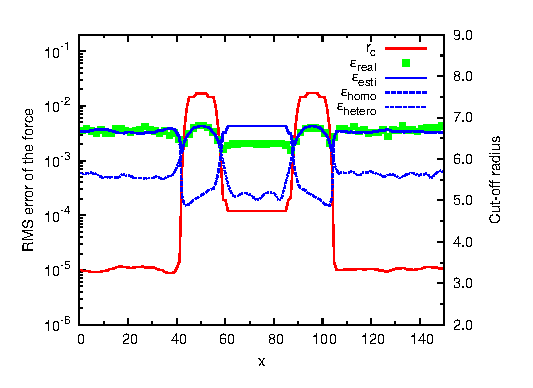
\includegraphics[]{fig/t0.85-n16000-adapt-e0.0045-extend/rcut.and.error.eps}
  \caption{ The RMS force error distribution of the 16000
    Lennard-Jones particle system at $T^\ast=0.85$ with adaptive
    cut-off radius. The control error $\mathcal E^\ast_{\textrm{C}}$
    is the same as the maximum error in the uniform cut-off simulation
    with $r_c^\ast=7.5$.  The resulting cut-off radius distribution is
    presented by the red line. All other notations are the same as
    Fig.~\ref{fig:tmp2}.}
  \label{fig:tmp3}
\end{figure}


In Fig. \ref{fig:tmp4}, the red solid line presents the $x$ component
correction force that is calculated every 40 time steps. The $y$ and
$z$ components are not shown because their magnitudes are negligible.
On the left interface, the correction force is along the positive
direction of $x$ axis, namely poiting right.  On the right interface,
the correction force is of the same maganitude but poiting
left. Therefore, the liquid density should be higher and the vapor
density should be lower than the corresponding uniform cut-off
simulation.  The real error (in green square) and the estimated
homogeneity error (in blue solid line) are all presented in
Fig. \ref{fig:tmp4}.  Cleary, the real error follows the homogeneity
error across the simulation region, which implies the contribution of
the inhomogeneity error is successfully removed, or is at least
negligible. In the bulk liquid region, the homogeneity error is
slightly overestimated, which is the same as the uniform and adaptive
cut-off simulations.

% Clearly the contribution of the inhomogeneity
% error is successfully removed, because the estimate of homogeneity
% error follows the real error perfectly in the interfacial regions.  In
% the bulk liquid region, the homogeneity error is slightly
% overestimated, which is the same as the uniform and adaptive cut-off
% simulations.

\begin{figure}
  \centering
  % 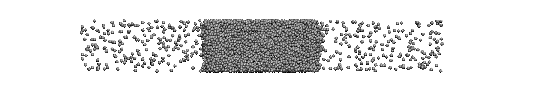
\includegraphics[scale=1]{fig/t0.85-n16000-rc07.5uni/confout-02.eps}
  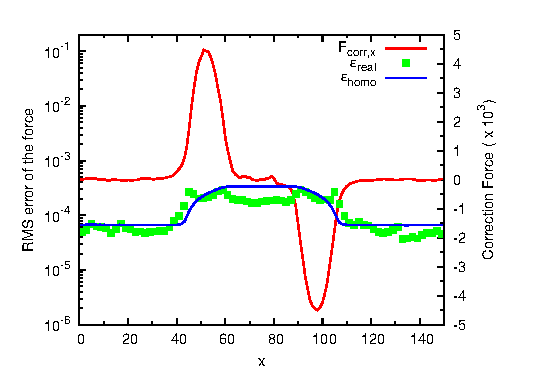
\includegraphics[]{fig/t0.85-n16000-fcorr-rc07.5-feq0200/fcorr.and.error.eps}
  \caption{ The RMS force error distribution of the 16000
    Lennard-Jones particle system at $T^\ast=0.85$ with long-range
    force correction, i.e. eqn. \eqref{eqn:define-fcorr}. The cut-off
    radius is $r^\ast_c = 7.5$. The $x$ component of the correction
    force is presented by the solid red line. The green squares
    present the real error. The solid blue line presents the estimated
    homogeneity error. }
  \label{fig:tmp4}
\end{figure}


% As mentioned before, form Fig. \ref{fig:tmp2}, the error dominates at
% the interfacial regions. The error estimate is sharp in these
% regions. While in the bulk regions, the error estimate is not sharp,
% but still acceptable. By the adapt cut-off radius MD, the resulting
% distribution (averaged on $y$ and $z$ directions) of cut-off radius is
% given in Fig. \ref{fig:tmp3}. In the interfacial regions, the cut-off
% radius is adapted to $r_c^\ast = 7.5$. In the bulk liquid and vapor
% regions, the cut-off radii are approximatly $5.0$ and $3.5$.  The
% resulting error distribution is ploted in FIg. \ref{fig:tmp4}. It is
% clear that the error is comparatively uniformly distributed in the
% space. The estimate inhomogeneity error is also dominant at the
% interfacial region, while the homogeneous error dominants in the bulk
% regions.  Since the computational cost is proportional to $r_c^3$,
% comparing with a simulation using uniform cut-off radius $7.5$, the
% adaptive cut-off simulation saves 3.4 times and 9.8 times
% computational cost, respectively. In total, the adaptive cut-off
% radius method save 50\% of the computational cost.

% We test the uniform and adaptive cut-off methods as well as the
% correction force method in the mentioned liquid vapor equilibrium
% system.

To test the effectiveness of the proposed adaptive cut-off and
long-range force correction methods, we measure the liquid-vapor
equilibrium density and the surface tension defined by
\begin{align}
  \gamma = \frac12 \int_{L_x}
  \bigg[\,
  p_x(x) - \frac{p_y(x) + p_z(x)}{2}
  \,\bigg]
  \,\d dx.
\end{align}
Where $p_x$, $p_y$ and $p_z$ are $x$, $y$ and $z$ component of the
pressure. The convergence of the properties of interest with respect
to the cut-off radius is considered.  For the adaptive cut-off
simulation, the ``cut-off radius'' means the largest cut-off radius
used in the simulation region. 

\begin{figure}
  \centering
  % 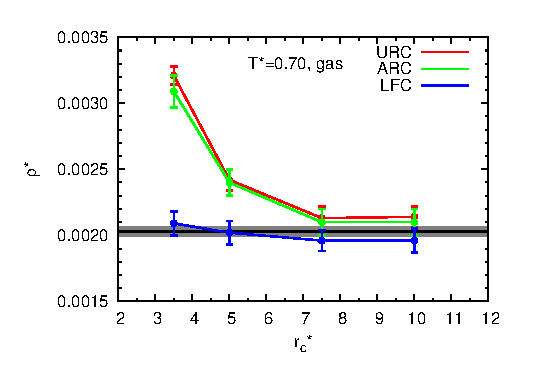
\includegraphics[width=0.42\textwidth]{fig/converge.new/t0.70.gas.eps} 
  % 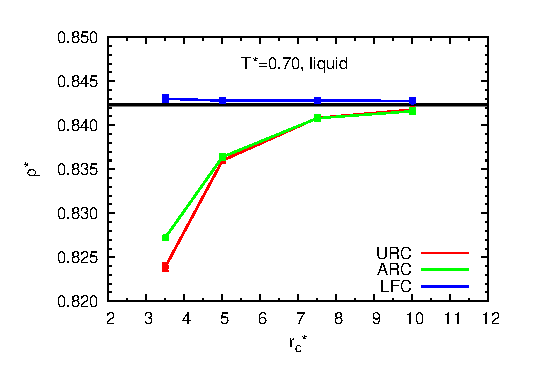
\includegraphics[width=0.42\textwidth]{fig/converge.new/t0.70.liquid.eps} 
  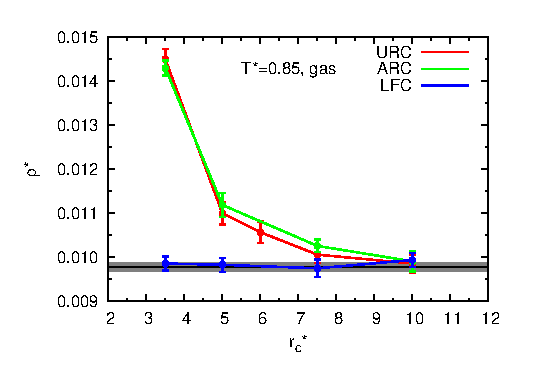
\includegraphics[width=0.49\textwidth]{fig/converge.new/t0.85.gas.eps} 
  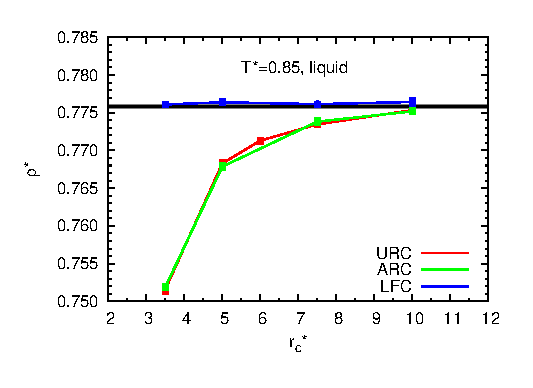
\includegraphics[width=0.49\textwidth]{fig/converge.new/t0.85.liquid.eps} 
  % 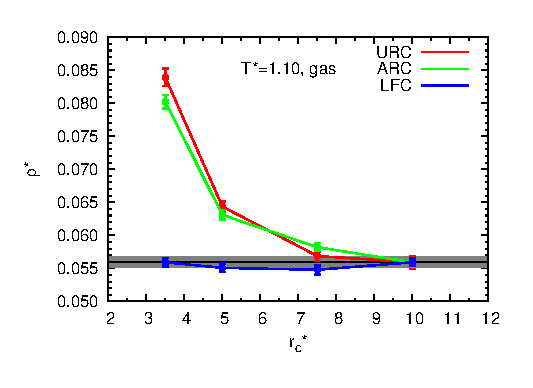
\includegraphics[width=0.42\textwidth]{fig/converge.new/t1.10.gas.eps} 
  % 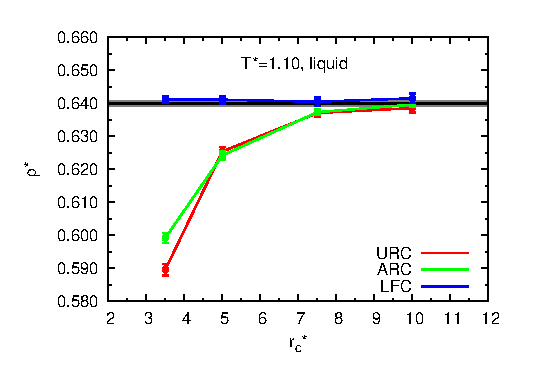
\includegraphics[width=0.42\textwidth]{fig/converge.new/t1.10.liquid.eps} 
  % 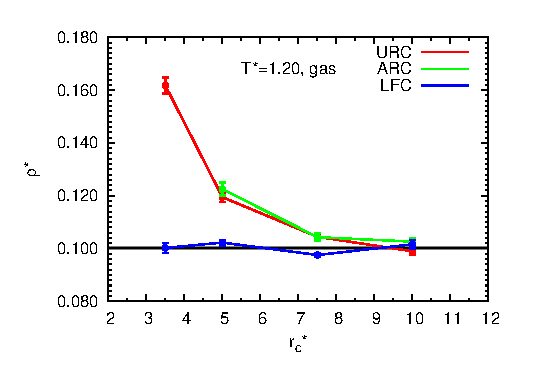
\includegraphics[width=0.42\textwidth]{fig/converge.new/t1.20.gas.eps} 
  % 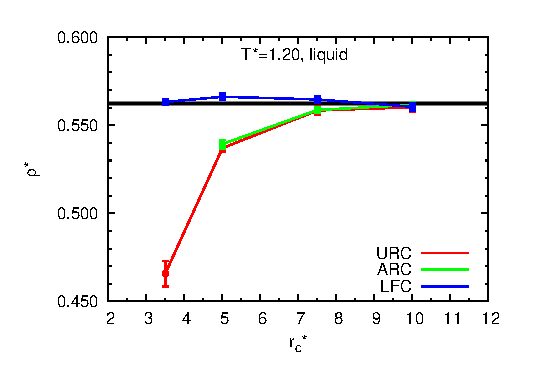
\includegraphics[width=0.42\textwidth]{fig/converge.new/t1.20.liquid.eps} 
  % 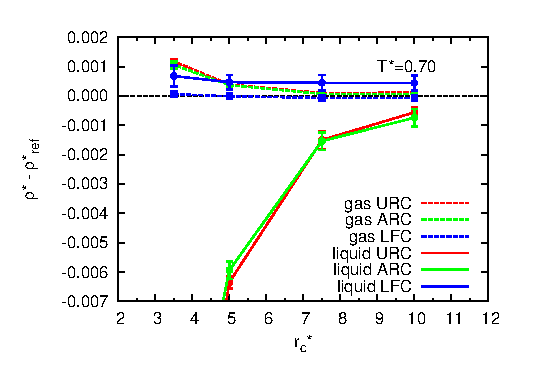
\includegraphics[width=0.49\textwidth]{fig/converge.new/t0.70.eps} 
  % 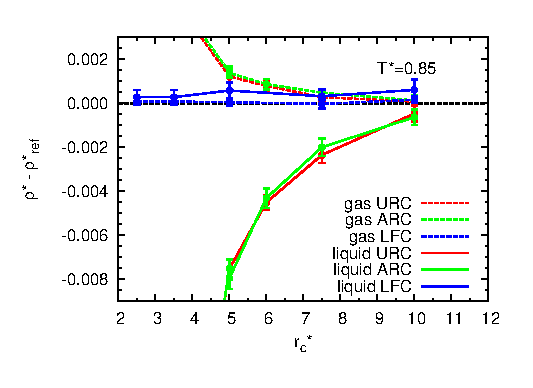
\includegraphics[width=0.49\textwidth]{fig/converge.new/t0.85.eps} 
  % 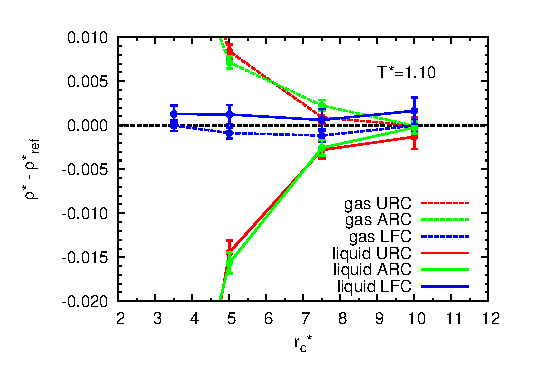
\includegraphics[width=0.49\textwidth]{fig/converge.new/t1.10.eps} 
  % 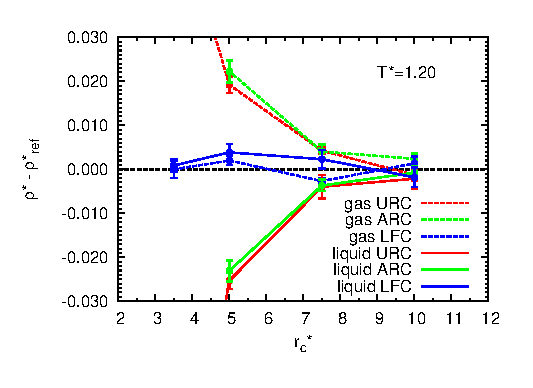
\includegraphics[width=0.49\textwidth]{fig/converge.new/t1.20.eps} 
  \caption{$T^\ast = 0.85$. The convergence of the equilibrium gas and
    liquid densities with respect to the cut-off radius. All densities
    are compared with the refence value (black solid line), namely,
    the liquid and vapor densities meansured with a uniform cut-off
    radius $r_c^\ast=13$. The gray region denotes the statistcal
    uncertainty of the reference value.  This figure presents the
    results of three methods, namely the uniform cut-off (URC), the
    adaptive cut-off (ARC) and the force correction (LFC) method. }
  \label{fig:tmp5}
\end{figure}

\begin{figure}
  \centering
  % 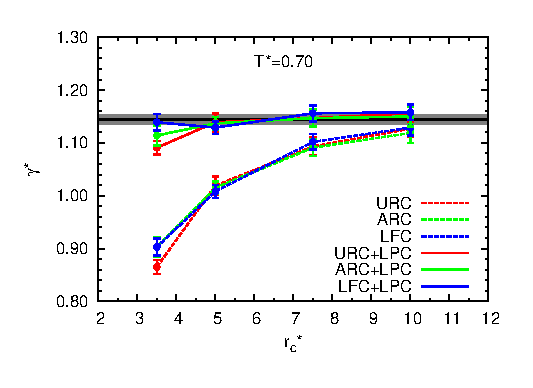
\includegraphics[width=0.49\textwidth]{fig/converge.new/tension.t0.70.eps} 
  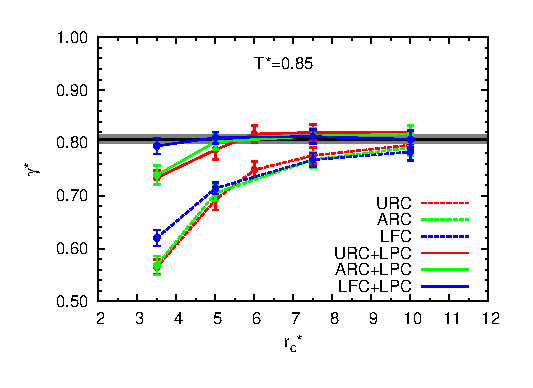
\includegraphics[width=0.49\textwidth]{fig/converge.new/tension.t0.85.eps} 
  % 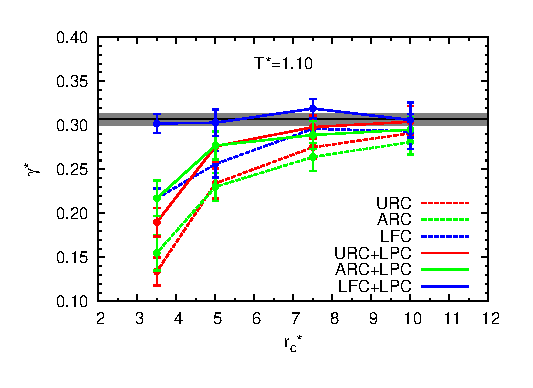
\includegraphics[width=0.49\textwidth]{fig/converge.new/tension.t1.10.eps} 
  % 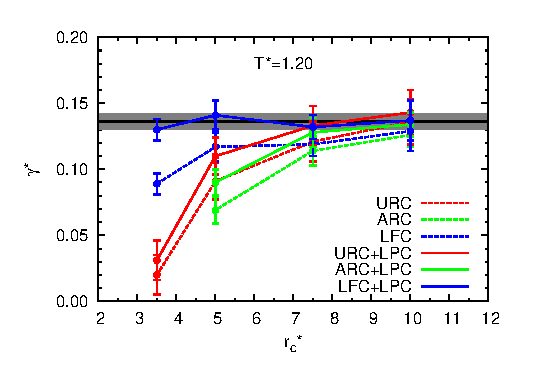
\includegraphics[width=0.49\textwidth]{fig/converge.new/tension.t1.20.eps} 
  \caption{$T^\ast = 0.85$. The convergence of the surface tension
    with respect to the cut-off radius.  This figure presents the
    results of three methods, namely the uniform cut-off (URC), the
    adaptive cut-off (ARC) and the long-range force correction (LFC)
    method.  The results with and without long-range pressure
    correction (LPC) are shown together for comparison. The reference
    surface tensions, shown by solid black lines, are measured by the
    uniform cut-off method with $r_c^\ast=13$ using LPC.}
  \label{fig:tmp6}
\end{figure}

\begin{table}
  \centering
  \caption{
    $T^\ast = 0.85$. The maximum RMS force error and computational cost of 
    three methods, namely the uniform cut-off
    (URC), the adaptive cut-off (ARC) and the long-range
    force correction (LFC) method.
    The computational cost is the number of pairwise interaction 
    measurements, which should be mashine-independent.
  }\label{tab:tmp1}
  \begin{tabular*}{0.50\textwidth}{c|@{\extracolsep{\fill}}ccc}\hline\hline
    $r^\ast_{c}$ & \textrm{method} & $\max\mathcal E^\ast$ & Cost($\times 10^{-6}$) \\ \hline
     &\textrm{URC} & $8.6\times 10^{-2}$ & 2.9 \\
 3.5 &\textrm{ARC} & $8.6\times 10^{-2}$ & 1.9 \\
     &\textrm{LFC} & $1.4\times 10^{-2}$ & 3.1 \\\cline{1-4}
     &\textrm{URC} & $2.2\times 10^{-2}$ & 7.8 \\
 5.0 &\textrm{ARC} & $2.2\times 10^{-2}$ & 4.5 \\
     &\textrm{LFC} & $1.9\times 10^{-3}$ & 7.9 \\\cline{1-4}
 6.0 &\textrm{URC} & $1.1\times 10^{-2}$ & 13 \\\cline{1-4}
     &\textrm{URC} & $4.5\times 10^{-3}$ & 24 \\
 7.5 &\textrm{ARC} & $4.3\times 10^{-3}$ & 12 \\
     &\textrm{LFC} & $2.3\times 10^{-4}$ & 24 \\\cline{1-4}
     &\textrm{URC} & $1.4\times 10^{-3}$ & 53 \\
10.0 &\textrm{ARC} & $1.4\times 10^{-3}$ & 26 \\
     &\textrm{LFC} & $5.3\times 10^{-5}$ & 53 \\ \hline\hline
  \end{tabular*}
\end{table}


% \begin{table}
%   \centering
%   \caption{
%     The maximum RMS force error and computational cost of 
%     three methods, namely the uniform cut-off
%     (URC), the adaptive cut-off (ARC) and the long-range
%     force correction (LFC) method.
%     The computational cost is the number of pairwise interaction 
%     measurements, which should be mashine-independent.
%   }\label{tab:tmp1}
%   \begin{tabular*}{0.50\textwidth}{c|c|@{\extracolsep{\fill}}ccc}\hline\hline
%     $T^\ast$ &$r^\ast_{c}$ & \textrm{method} & $\max\mathcal E^\ast$ & Cost($\times 10^{-6}$) \\ \hline
% %     & 3.5 &\textrm{LFC} & $1.4\times 10^{-2}$ & 3.4 \\\cline{2-5}
% %     &     &\textrm{URC} & $2.5\times 10^{-2}$ & 7.9 \\
% %     & 5.0 &\textrm{ARC} & $2.4\times 10^{-2}$ & 4.6 \\
% %     &     &\textrm{LFC} & $2.0\times 10^{-3}$ & 8.8 \\\cline{2-5}
% %     &     &\textrm{URC} & $4.9\times 10^{-3}$ & 27 \\
% % 0.70& 7.5 &\textrm{ARC} & $4.9\times 10^{-3}$ & 13 \\
% %     &     &\textrm{LFC} & $2.5\times 10^{-4}$ & 27 \\\cline{2-5}
% %     &     &\textrm{URC} & $1.6\times 10^{-3}$ & 59 \\
% %     &10.0 &\textrm{ARC} & $1.6\times 10^{-3}$ & 29 \\
% %     &     &\textrm{LFC} & $5.8\times 10^{-5}$ & 59 \\ \hline\hline
%     &     &\textrm{URC} & $8.6\times 10^{-2}$ & 2.9 \\
%     & 3.5 &\textrm{ARC} & $6.7\times 10^{-2}$ & 2.1 \\
%     &     &\textrm{LFC} & $1.4\times 10^{-2}$ & 3.1 \\\cline{2-5}
%     &     &\textrm{URC} & $2.2\times 10^{-2}$ & 7.8 \\
%     & 5.0 &\textrm{ARC} & $1.9\times 10^{-2}$ & 4.6 \\
%     &     &\textrm{LFC} & $1.9\times 10^{-3}$ & 7.9 \\\cline{2-5}
%     &     &\textrm{URC} & $4.5\times 10^{-3}$ & 24 \\
% 0.85& 7.5 &\textrm{ARC} & $4.3\times 10^{-3}$ & 12 \\
%     &     &\textrm{LFC} & $2.3\times 10^{-4}$ & 24 \\\cline{2-5}
%     &     &\textrm{URC} & $1.4\times 10^{-3}$ & 53 \\
%     &10.0 &\textrm{ARC} & $1.4\times 10^{-3}$ & 26 \\
%     &     &\textrm{LFC} & $5.3\times 10^{-5}$ & 53 \\ \hline\hline
%   \end{tabular*}
% %   \begin{tabular*}{0.49\textwidth}{c|c|@{\extracolsep{\fill}}ccc}\hline\hline
% %     $T^\ast$ &$r^\ast_{c}$ & \textrm{method} & $\max\mathcal E^\ast$ & Cost($\times 10^{-6}$) \\ \hline
% %     & 3.5 &\textrm{LFC} & $1.3\times 10^{-2}$ & 3.8 \\\cline{2-5}
% %     &     &\textrm{URC} & $1.5\times 10^{-2}$ & 5.6 \\
% %     & 5.0 &\textrm{ARC} & $1.5\times 10^{-2}$ & 3.2 \\
% %     &     &\textrm{LFC} & $1.7\times 10^{-3}$ & 9.9 \\\cline{2-5}
% %     &     &\textrm{URC} & $3.3\times 10^{-3}$ & 17 \\
% % 1.10& 7.5 &\textrm{ARC} & $3.5\times 10^{-3}$ & 8.8 \\
% %     &     &\textrm{LFC} & $1.8\times 10^{-4}$ & 18 \\\cline{2-5}
% %     &     &\textrm{URC} & $1.1\times 10^{-3}$ & 39 \\
% %     &10.0 &\textrm{ARC} & $1.0\times 10^{-3}$ & 19 \\
% %     &     &\textrm{LFC} & $4.2\times 10^{-5}$ & 39 \\ \hline\hline
% % %     & 3.5 &\textrm{LFC} & $1.2\times 10^{-2}$ & 1.8 \\\cline{2-5}
% % %     &     &\textrm{URC} & $1.1\times 10^{-2}$ & 4.2 \\
% % %     & 5.0 &\textrm{ARC} & $1.0\times 10^{-2}$ & 2.8 \\
% % %     &     &\textrm{LFC} & $1.5\times 10^{-3}$ & 4.6 \\\cline{2-5}
% % %     &     &\textrm{URC} & $2.5\times 10^{-3}$ & 14 \\
% % % 1.20& 7.5 &\textrm{ARC} & $2.4\times 10^{-3}$ & 7.7 \\
% % %     &     &\textrm{LFC} & $1.5\times 10^{-4}$ & 14 \\\cline{2-5}
% % %     &     &\textrm{URC} & $8.2\times 10^{-4}$ & 30 \\
% % %     &10.0 &\textrm{ARC} & $8.3\times 10^{-4}$ & 17 \\
% % %     &     &\textrm{LFC} & $3.3\times 10^{-5}$ & 31 \\\hline\hline
% %   \end{tabular*}
% \end{table}

In the Fig. \ref{fig:tmp5} and Fig. \ref{fig:tmp6}, the convergence of
the equilibrium liquid/vapor densities and surface tension are
investigated with respect to the increasing cut-off radius. The red,
green and blue points with error bars denote the results of uniform,
adaptive cut-off methods and the long-range force correction,
respectively.  In Fig. \ref{fig:tmp5}, all densities are compared with
the reference value measured by the uniform cut-off simulation of
$r_c^\ast = 13$, with the statistcal uncertainty denoted by the gray
region. The densities are connected by the the solid lines to guide
the eyes.  In Fig. \ref{fig:tmp6}, the direct measures of surface
tension (data points connected by the dashed lines) are presented with
pressure corrected surface tension (data points connected by solid
lines).  The same as the reference densities, the reference surface
tension is measured by uniform cut-off simulations at $r_c^\ast = 13$
with long-range pressure correction.  Table \ref{tab:tmp1} presents
the maximum RMS force error and the computational expense of the
mentioned methods at different cut-off radii. The computational cost
is given by the average number of pairwise interactions calculated by
the program, which is platform independent and serves as a good bench
mark.

% In the higher
% temperature cases, the thermodynamic flucuation of the system is
% stronger. Therefore, the meansurement of densities and surface tension
% are less accurate.
% At $T^\ast = 0.70$, the gas
% density converges much faster than the liquid density, while at
% $T^\ast = 1.20$, the gas and liquid densities almost converges at the
% same speed, see Fig. \ref{fig:tmp5}.

The liquid and gas densities of the uniform and the adaptive cut-off
methods are almost identical at the same cut-off radius, see
Fig. \ref{fig:tmp5}. This observation is also true for the surface
tension, see Fig. \ref{fig:tmp6}. This indicates that controlling the
maximum of force error (see Tab. \ref{tab:tmp1}) and introducing
larger homogeneous force error in the bulk liquid/gas regions will not
disturb the accuracy of the equilibrium densities and surface tension.
The adaptive cut-off method roughly saves 1/3 -- 1/2 of the
computational cost (see Tab. \ref{tab:tmp1}). The efficiency benefit
of the adaptive cut-off depends on the property of the system: if the
bulk regions dominate the system, and the inhomogeneity produces large
interfacial force error, then the adaptive cut-off will save a lot of
computational expense. On the other hand, if the interfacial region is
computationally intensive, the adaptive cut-off will not improve the
efficency greatly.

The long-range force correction method presents a much better density
convergence than the uniform and adaptive cut-off simulations: the
equilibrium densities converge when the cut-off radius is only 3.5,
see Fig. \ref{fig:tmp5}. The maximum RMS force error is reduced by roughly
one order of maganitude, comparing to the uniform and adaptive cut-off
methods, see Tab. \ref{tab:tmp1}. The computationally cost of the
force correction method is the same as the uniform cut-off methods at
the same cut-off radius. 

% With the
% same cut-off radius, the computational cost of the force correction is
% nearly the same as the uniform cut-off methods, see
% Tab. \ref{tab:tmp1}, and at the same time, the force accuracy is more
% than one order of maganitude better.

% However, the maximum
% force error of the force correction method is reduced by about one
% order of maganitude.
% We also observe that the liquid densities are systemetically higher
% than the reference results. This fact will be discussed later by
% comparing with literature results.

The surface tension result of the force correction without pressure
correction is only slightly better than the uniform and adaptive
cut-off methods without pressure correction, see Fig. \ref{fig:tmp6}.
With the long-range pressure correction, the convergence of the
surface tension of all methods are greatly improved.  The force
correction method converges at $r_c^\ast = 3.5$, and the
uniform/adaptive cut-off methods converge at $r_c^\ast = 6.0$.  The
discrepancy between the corrected and uncorrected tension is the
amount of the correction, which decreases with the increasing cut-off
radius. However, even at $r_c^\ast=10$, this correction is not
negligible. 

Comparing the results of the force correction method at $r_c^\ast =
3.5$ and uniform cut-off radius method at $r_c^\ast = 6.0$, the force
accuracy of the former method is worse than the later (see
Tab. \ref{tab:tmp1}), but the equilibrium density accuracy is better than
the later, and surface tension is as good as the later (see
Fig. \ref{fig:tmp5} and \ref{fig:tmp6}).
% In the force correction simulation, the
% inhomogeneity error is screened out and the force error term is
% dominated by the homogeneity error. And in the uniform cut-off
% simulation the force error is dominated by the inhomogeneity error.
Since the homogeneity error dominates in the former simulation and the
inhomogeneity error dominates in the later, the above observation
indicates different natures of error play different roles in the
simulations.  The homogeneity error is actually the variation of the
corrected error force that has a vanished mean, see
Eqn. \eqref{eqn:mean-fcorr}. This implies that the corrected error
force may point to any direction with the same probability, and may be
cancelled by itself in a long time average.  The inhomogeneity error,
in contrast, stems from the non-vanishing mean value of the error
force, which is alway pointing at one certain direction (the opposite
direction of the density gradient), and has low  oppotunity to be
self-cancelled.


% To verify our simulations, we compare our results in
% Tab. \ref{tab:comparison} with a wide range of results reported by
% literature~\cite{janecek2006long, lotfi1992vapour,
%   errington2003evaluating, ismail2007application}

% We list in Tab. \ref{tab:comparison} a wide range of results reported
% by literature~\cite{janecek2006long, lotfi1992vapour,
%   errington2003evaluating, ismail2007application}, as well as our
% uniform ($r_c^\ast = 13$) and force correction ($r_c^\ast = 5.0$)
% results for comparison. The abbreviations in the table are explained
% in the caption. The MC/LEC, MD/Ewald and our methods are direct
% simulation of the inhomogeneous system. The MD/Npt+test particle and
% MC/GC-TMMC methods are simulation of homogeneous systems that do not
% have the difficulties of inhomogeneity, and are believed to be more
% precise than direct simulations~\cite{shen2007comparative}.

% \begin{table}
%   \centering
%   \caption{Equilibrium densities and surface tension comparision 
%     with various literature results: Monte Carlo with long-range
%     energy correction (MC/LEC)~\cite{janecek2006long}, Npt+test
%     particle molecular dynamics (MD/Npt+test particle)~\cite{lotfi1992vapour},
%     grand-canonical transition-matrix Monte Carlo (MC/GC-TMMC)~\cite{errington2003evaluating},
%     molecular dynamics with dispersion term calculated by the Ewald
%     summation (MD/Ewald)~\cite{ismail2007application}
%     and uniform cut-off (URC) and long-range force correction (LFC) molecular dynamics
%     proposed by this work. The surface tensions of this work are
%     corrected by the long-range pressure correction.
%     The cut-off radius of the Ewald summation is for the real space.
%   }
%   \label{tab:comparison}
%   \begin{tabular*}{0.99\textwidth}{@{\extracolsep{\fill}}clllllc}\hline\hline
%   % \begin{tabular}{cccc|cccc}\hline\hline
%     $T^\ast$ & Method & $r_c^\ast$ & $\rho^\ast_{\textrm{liq}}$ & $\rho^\ast_{\textrm{vap}}$ & $\gamma^\ast$ & Source \\\hline
%     0.70 & MC/LEC               & 2.5      & 0.842(1)    & 0.0021(2)   & 1.21(2)   & \cite{janecek2006long}\\
%     0.70 & MD/Npt+test particle & 5.0      & 0.84266(18) & 0.00193(10) & -         & \cite{lotfi1992vapour}\\
%     0.70 & MC/GC-TMMC           & 1/2 box  & 0.8424(13)  & 0.001992(2) & 1.182(10) & \cite{errington2003evaluating}\\
%     % 0.70 & MD/Ewald             & 5.0(real)& 0.8414(1)   & 0.0020(0)   & 1.141(11) & \cite{ismail2007application}\\
%     0.70 & MD/URC               & 13.0     & 0.8423(2)   & 0.0020(0)   & 1.128(10) & this work \\
%     % 0.70 & MD/LFC               & 5.0      & 0.8424(2)   & 0.0021(1)   & 1.145(11) & this work \\\hline
%     0.70 & MD/LFC               & 3.5      & 0.8430(4)   & 0.00209(9)  & 1.139(16) & this work \\\hline
%     0.85 & MD/Npt+test particle & 5.0      & 0.77623(25) & 0.00970(22) & -         & \cite{lotfi1992vapour}\\
%     0.85 & MC/GC-TMMC           & 1/2 box  & 0.7760(10)  & 0.009611(9) & 0.837(2)  & \cite{errington2003evaluating}\\
%     % 0.85 & MD/Ewald             & 5.0(real)& 0.7750(1)   & 0.0098(0)   & 0.818(15) & \cite{ismail2007application}\\
%     0.85 & MD/URC               & 13.0     & 0.7758(3)   & 0.0098(1)   & 0.794(09) & this work \\
%     % 0.85 & MD/LFC               & 5.0      & 0.7760(4)   & 0.0098(1)   & 0.823(21) & this work\\\hline
%     0.85 & MD/LFC               & 3.5      & 0.7761(3)   & 0.00986(16) & 0.794(15) & this work\\\hline
%     1.10 & MC/LEC               & 2.5      & 0.642(1)    & 0.054(1)    & 0.33(2)   & \cite{janecek2006long}\\
%     1.10 & MD/Npt+test particle & 5.0      & 0.6401(12)  & 0.0533(14)  & -         & \cite{lotfi1992vapour}\\
%     1.10 & MC/GC-TMMC           & 1/2 box  & 0.6410(7)   & 0.05485(5)  & 0.343(2)  & \cite{errington2003evaluating}\\
%     % 1.10 & MD/Ewald             & 5.0(real)& 0.6383(1)   & 0.0553(0)   & 0.302(11) & \cite{ismail2007application}\\
%     1.10 & MD/URC               & 13.0     & 0.6399(9)   & 0.0560(8)   & 0.300(07) & this work\\
%     % 1.10 & MD/LFC               & 5.0      & 0.6405(9)   & 0.0553(6)   & 0.293(9)  & this work\\ \hline
%     1.10 & MD/LFC               & 3.5      & 0.6411(10)   & 0.0559(6)   & 0.302(11)  & this work\\ \hline
%     1.20 & MC/LEC               & 2.5      & 0.566(1)    & 0.109(2)    & 0.16(2)   & \cite{janecek2006long}\\
%     1.20 & MD/Npt+test particle & 5.0      & 0.5661(22)  & 0.0987(16)  & -         & \cite{lotfi1992vapour}\\
%     % 1.20 & MD/Ewald             & 5.0(real)& 0.5627(2)   & 0.0942(0)   & 0.156(14) & \cite{ismail2007application}\\
%     1.20 & MD/URC               & 13.0     & 0.5624(11)  & 0.1002(5)   & 0.131(6) & this work\\
%     % 1.20 & MD/LFC               & 5.0      & 0.5651(22)  & 0.0987(11)  & 0.136(17) & this work\\
%     1.20 & MD/LFC               & 3.5      & 0.5632(14)  & 0.1002(19)  & 0.130(8) & this work\\
%     \hline\hline
%   % \end{tabular}
%   \end{tabular*}
% \end{table}


% The reason is the corrected error force has a varnished mean
% value (, so it may point to any
% direction with the same possibility.  With the same cut-off radius,
% the computational cost of the force correction and uniform cut-off
% methods are nearly the same, see Tab. \ref{tab:tmp1}. However, the
% maximum force error of the force correction method is about one order
% of maganitude more precise, comparing with the uniform cut-off
% simulations.


% The convergence of the surface tension with respect to the cut-off
% radius is shown in the Fig. \ref{fig:tmp6}. The color notation is the
% same as Fig. \ref{fig:tmp5}.  Surface tensions measured with and
% without inhomogeneous pressure correction are connected by solid and
% dashed lines, respectively.  The reference surface tension is
% presented by the black solid lines. The inhomogeneous pressure
% correction improve the surface tention measurement greatly. The
% discrepancy between the corrected and uncorrected pressure is the
% value of the correction, which decreases with increasing cut-off
% radius. However, even at $r_c^\ast=10$, the correction is not
% negligible for $T^\ast = 0.70$ and $T^\ast = 0.85$. At higher
% temperature, the statistical uncertainty gets larger, and better
% convergence is achieved at small cut-off radius.

% Although the force correction is a
% little better, no substential difference between the different
% simulation methods is observed. However, the With the
% pressure correction, the result is acceptable at cut-off 5.0 and
% satisfactorily converged at cut-off 7.5.







% The equilibrium liquid and vapor densities with respect to
% the cut-off radius are presented in Fig. \ref{fig:tmp5}. For the
% adaptive cut-off simulation, the data points represent the largest
% cut-off radius used in the simulations. All the results are
% substracted by the reference results, which are calculated at uniform
% cut-off radius of 13, for a clear comparison. Solid and dashed lines
% are added to the data points of vapor and liquid densities
% respectively. For the uniform and adaptive cut-off simulations, the
% cut-off radii 5, 7.5 and 10 are considered. For the force correction,
% the cut-off 3.5 is investigated in addition. We perform simulations at
% different temperature: that are denoted in the plots.





% \begin{figure}
%   \centering
%   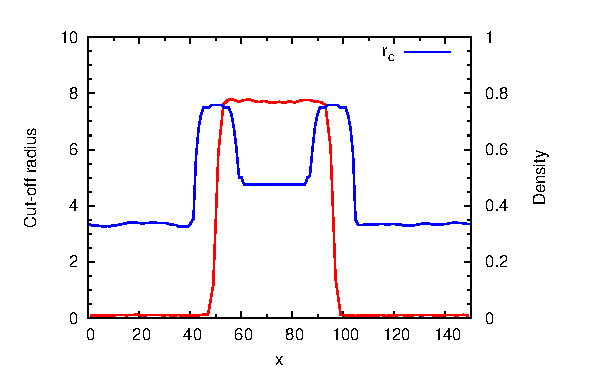
\includegraphics[]{fig/t0.85-n16000-adapt-e0.0045-extend/rcut.adapt.eps}
%   \caption{The adapted cut-off radius of the 16000 Lennard-Jones
%     particle system at $T^\ast=0.85$.}
%   \label{fig:tmp3}
% \end{figure}


% \begin{figure}
%   \centering
%   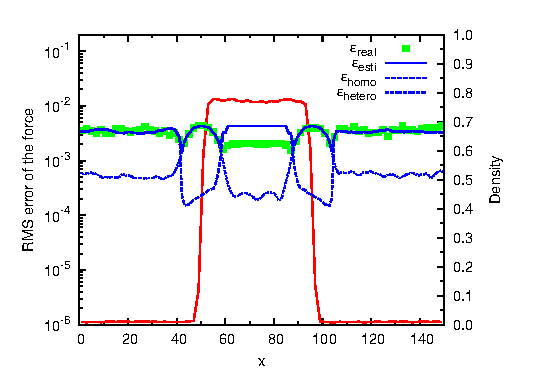
\includegraphics[]{fig/t0.85-n16000-adapt-e0.0045-extend/error.adapt.eps}
%   \caption{The error distribution of the adaptive-cut-off 16000
%     Lennard-Jones particle system at $T^\ast=0.85$.}
%   \label{fig:tmp4}
% \end{figure}


% \begin{figure}
%   \centering
%   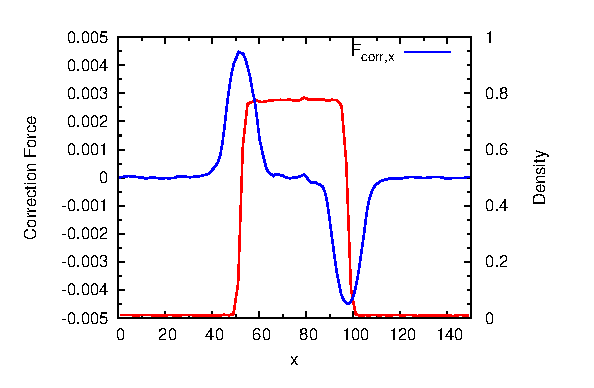
\includegraphics[]{fig/t0.85-n16000-fcorr-rc07.5-feq0200/fcorr.eps}
%   \caption{The correction force simulation of the 16000 Lennard-Jones
%     particle system at $T^\ast=0.85$.}
%   \label{fig:tmp3}
% \end{figure}


% \begin{figure}
%   \centering
%   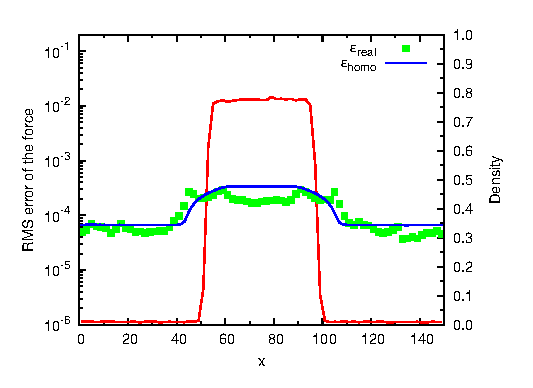
\includegraphics[]{fig/t0.85-n16000-fcorr-rc07.5-feq0200/error.fcorr.eps}
%   \caption{The correction force simulation of the adaptive-cut-off 16000
%     Lennard-Jones particle system at $T^\ast=0.85$.}
%   \label{fig:tmp4}
% \end{figure}








\subsection{Collision of nanoscale Lennard-Jones clusters}
\label{sec:tmp2.2}


\begin{figure}
  \centering
  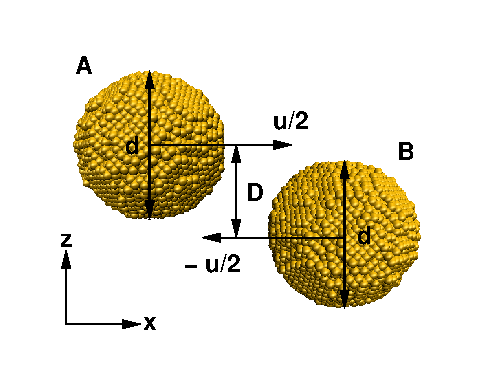
\includegraphics[]{fig/collision-init/init.2.eps}
  \caption{The initial setup of cluster $A$ and $B$. The initial
    velocity are equal in maganitude but on opposite direction.}
  \label{fig:tmp7}
\end{figure}

In this section, we test the adaptive cut-off method and the long-range force
correction method in a dynamical problem: collision of nanoscale
Lennard-Jones clusters. Two initial Lennard-Jones clusters, denoted by
$A$ and $B$, are setup in the simulation box, each of which contains
the same number of particles $N_A = N_B = 10792$, with a diameter of
$d^\ast\approx 27$. The initial velocity of the clusters are $\v u_A =
\frac12(u, 0, 0)$ and $\v u_B = -\frac12(u, 0, 0)$, see
Fig. \ref{fig:tmp7}. The impact parameter $D$ is defined by the $z$
corrdinate difference between the center of mass (COM) of the
clusters. The unitless impact factor defined by
\begin{align}
  x = \frac D d
\end{align}
is used to measure how far off-center the collision happens. If $x =
0$ the collision is head-on, while $x=1$ the collision is avoided.
Ref. \cite{kalweit2006collision} investigated a board range
combination of the velocity $u$ and impact factor $x$, and identified
three major collision modes: the coalescence, the streching seperation
and the shattering. The major modes were further classified into a
series submodes. In this paper, we want to study the how the collision
properties are affected by the force 
precision. Therefore, we focus on one special case: $u^\ast = 2.2$ and
$x^\ast = 0.6$, where the major collision mode is the coalescence, and a
poor precision of force calculation may lead to a wrong major
collision mode.

\begin{figure}
  \centering
  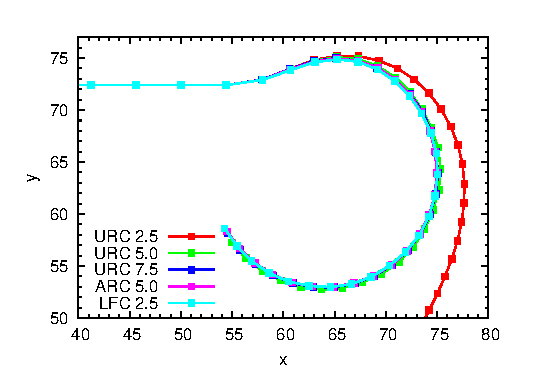
\includegraphics[]{fig/trajs.eps}
  \caption{The center of mass trajectory of cluster A. Uniform cut-off
    (URC) $r_c^\ast = 2.5,\ 5.0,\ 7.5$, adaptive cut-off (ARC) $r_c =
    5.0$ and long-range force correction (LFC) $r^\ast_c = 2.5$ are
    investigated.  The time interval between two neighboring squares
    on the trajectory is 4.  }
  \label{fig:tmp8}
\end{figure}

\begin{figure}
  \centering
  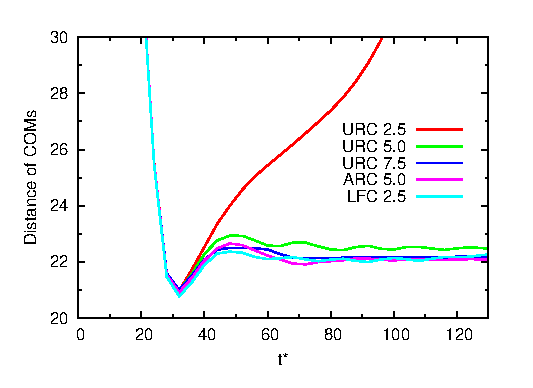
\includegraphics[]{fig/dists.eps}
  \caption{The COM distance between cluster $A$ and cluster $B$ versus
    time. Uniform cut-off (URC) $r_c^\ast = 2.5,\ 5.0,\ 7.5$, adaptive
    cut-off (ARC) $r_c = 5.0$ and long-range force correction (LFC)
    $r^\ast_c = 2.5$ are investigated.  }
  \label{fig:tmp9}
\end{figure}


In Fig. \ref{fig:tmp8} and \ref{fig:tmp9}, we present the trajectory
of COM of cluster $A$ and the COM distance between the two clusters,
respectively. Three different cut-off radii of uniform cut-off
simulation are considered. It is obvious that the trajectory of
$r_c^\ast = 2.5$ is completely wrong: two clusters seperate after
collision. The $r_c^\ast = 5.0$ trajectory is reasonably good, but the
COM distance converges only when $r_c^\ast = 7.5$. This means the
precision of force calculation is crucial in the study of collision
dynamics. Althougth the precision of the adaptive cut-off method with
$r_c^\ast = 5$ is the same as uniform cut-off $r_c^\ast = 5$, the former
produces better trajectory. The long-range force
correction method that gets rid of the inhomogeneity error also produces
correct trajectory, but the motion along the trajectory is somewhat
faster than other methods (see also the angular velocity in
Fig. \ref{fig:tmp11}).


\begin{figure}
  \centering
  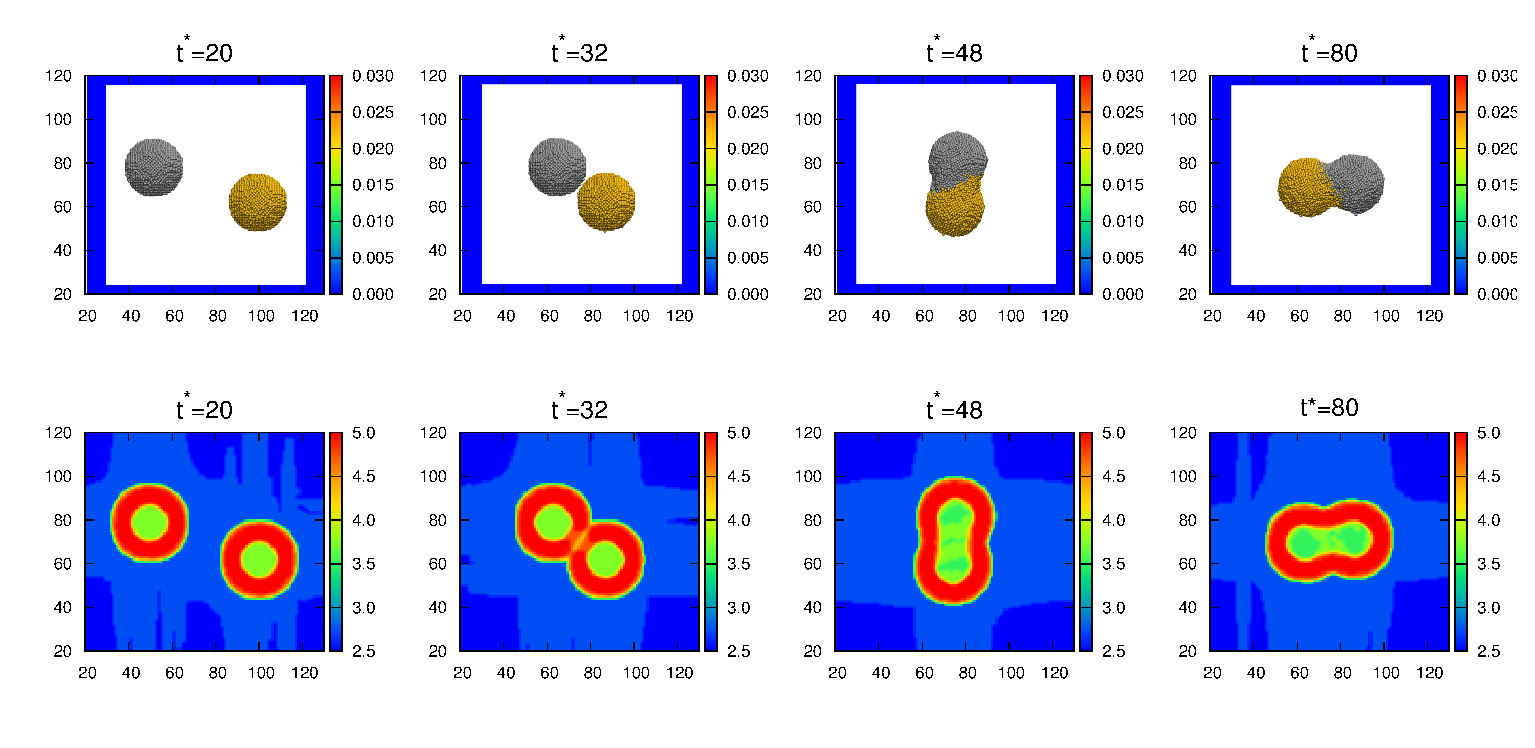
\includegraphics[width=0.90\textwidth]{fig/error-rcut-ball.eps} 
  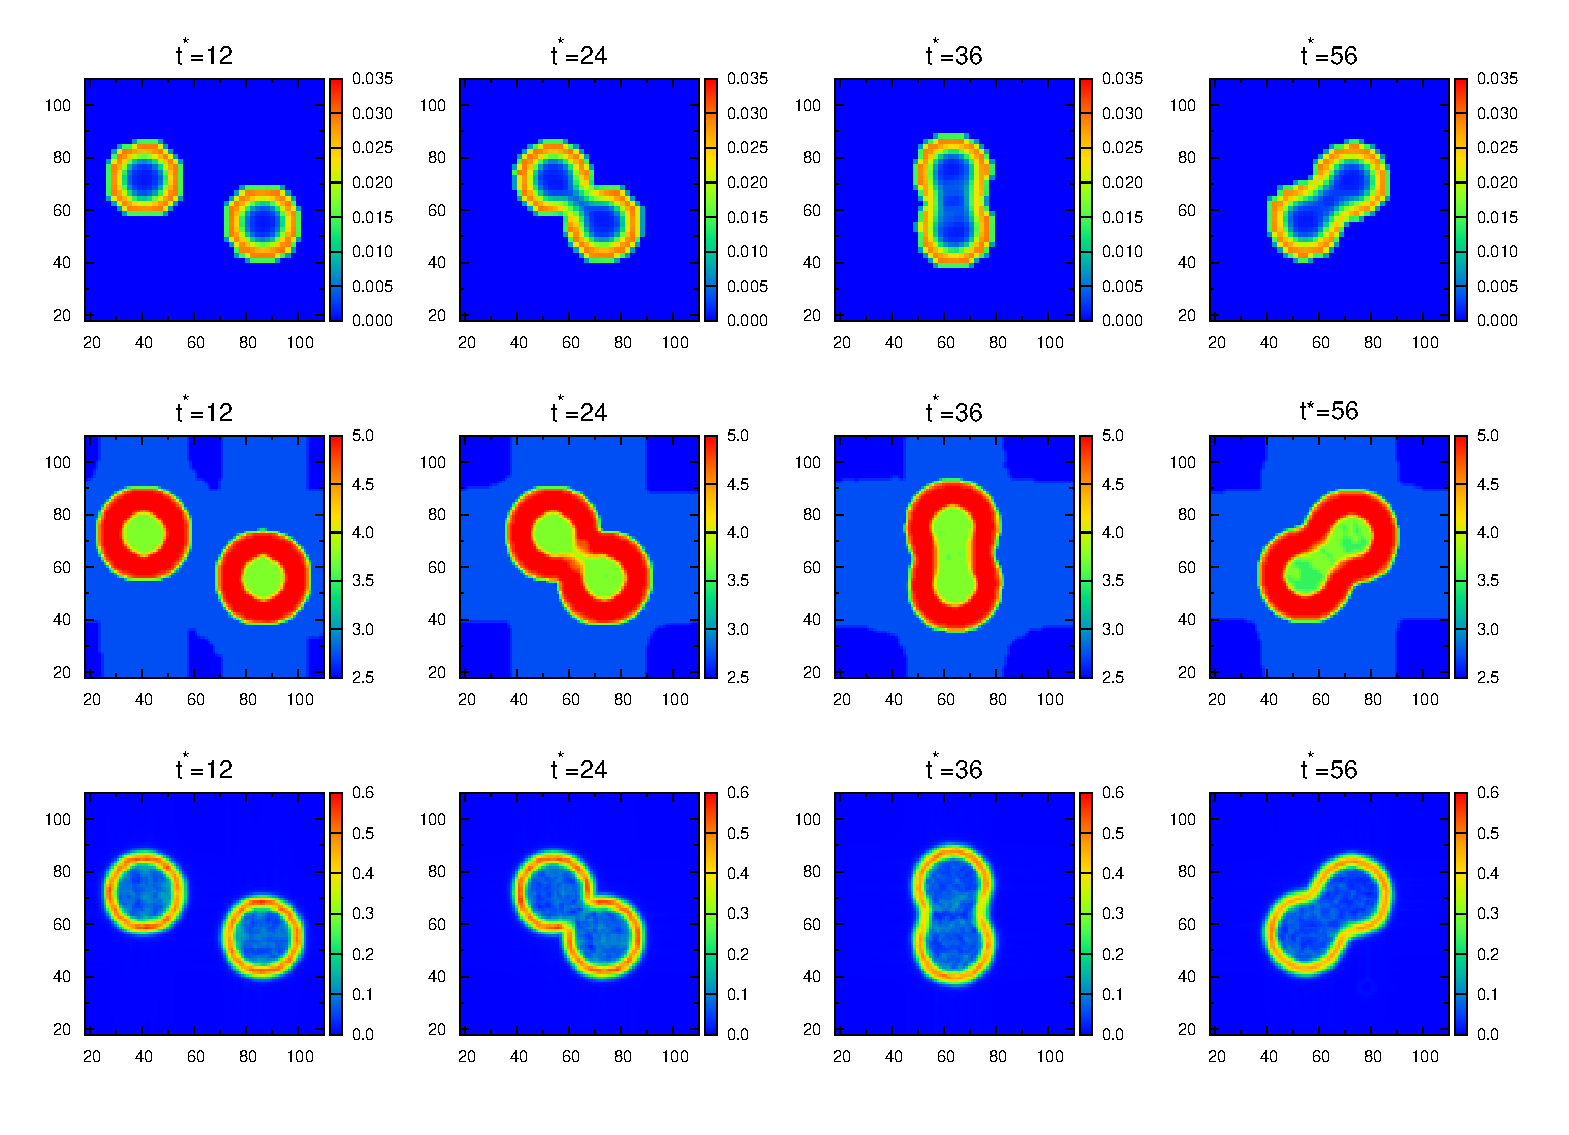
\includegraphics[width=0.90\textwidth]{fig/error-rcut.eps}
  \caption{The colliding clusters (the first row), the RMS force error
    distribution of uniform cut-off with $r_c^\ast = 5.0$ (the second
    row), the cut-off distribution of adaptive cut-off with $r_c^\ast
    = 5.0$ (the third row) and the magenitude of long-range force
    correction with $r_c^\ast = 2.5$ (the fourth row). The four
    columes corresponds to snap shots taken at $t^\ast = 12,\ 24,\
    36,\ 56$, respectively.  }
  \label{fig:tmp10}
\end{figure}

The RMS force error of uniform cut-off, the cut-off
distribution of adaptive cut-off and the magnitude of
the correction force of long-range force correction method
are plotted in Fig. \ref{fig:tmp10}.  The configuration of the two
clusters (colored in gray and yellow) are presented on top of the
figure for reference. The same as the liquid-vapor equilibrium
simulation, the force error dominates in the interfacial regions,
namely the boundaries of the clusters. Inside and outside the
clusters, the error is much lower. The cut-off distribution of the
adaptive cut-off method is updated every 200 time steps. The third row
of Fig. \ref{fig:tmp10} shows that the large cut-off region follows the cluster
boundaries perfectly. It is much border than the
large error region, because it is refined by Eqn. \eqref{eqn:rc-refine}
to keep track of the
possible moving of the clusters.  The correction force is calculated
every 10 time steps. From the fourth row 
of Fig. \ref{fig:tmp10}, it also follows the moving boundaries the colliding
clusters. In the bulk region of the clusters, the correction force is
neglectable. It is not efficient to calculate the correction force more
frequently, because
every force correction involves FFTs that are comparatively expensive
especially when the cut-off radius is small. 
In the present case, FFTs take up 50\% of the
total computational cost. 
% The FFTs are comparably more expensive than one step of MD simulation. 

\begin{figure}
  \centering
  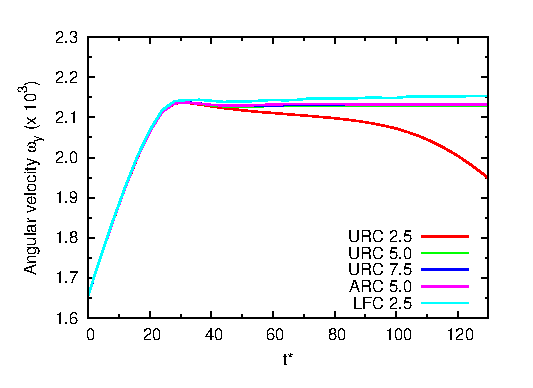
\includegraphics[]{fig/wy.eps}
  \caption{The angular velocity of cluster $A$ versus time. Uniform
    cut-off (URC) $r_c^\ast = 2.5,\ 5.0,\ 7.5$, adaptive cut-off (ARC)
    $r_c = 5.0$ and long-range force correction (LFC) $r^\ast_c = 2.5$
    are investigated.}
  \label{fig:tmp11}
\end{figure}

\begin{figure}
  \centering
  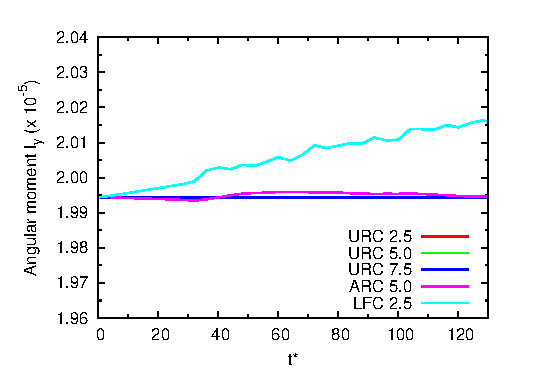
\includegraphics[]{fig/ly.eps}
  \caption{The angular moment of cluster $A$ versus time. Uniform
    cut-off (URC) $r_c^\ast = 2.5,\ 5.0,\ 7.5$, adaptive cut-off (ARC)
    $r_c = 5.0$ and long-range force correction (LFC) $r^\ast_c = 2.5$
    are investigated.}
  \label{fig:tmp12}
\end{figure}


The angular velocity is presented in Fig. \ref{fig:tmp11}. The force
correction result is not as precise as other simulations excluding
uniform $r_c = 2.5$ simulation. This probably because the value of the
correction force is updated every 10 time steps, so considering the
moving of the clusters, it is not the exactly up-to-date value.
% This because the correction force is
% not precise because it is calculated every \recheck{aaa} steps.
In the Fig. \ref{fig:tmp12} presents the angular moment, which should be
preserved during the simulations. All uniform simulations
preserve the angular moment perfectly. The angular moment of the
adaptive cut-off simulation, which does not precisly preserve the
Newton's third law, shows deviation but is still around the correct
value. However, the angular moment of the force correction simulation
deviates away from the correct value by 1 \% at $t^\ast = 130$.


\begin{figure}
  \centering
  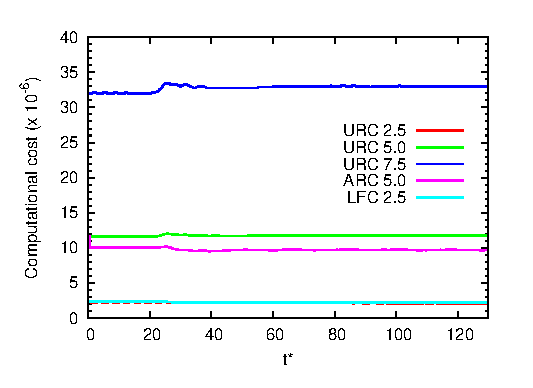
\includegraphics[]{fig/cost.eps}
  \caption{The computational cost versus time. Uniform
    cut-off (URC) $r_c^\ast = 2.5,\ 5.0,\ 7.5$, adaptive cut-off (ARC)
    $r_c = 5.0$ and long-range force correction (LFC) $r^\ast_c = 2.5$
    are investigated.}
  \label{fig:tmp13}
\end{figure}

The computational cost is given in Fig. \ref{fig:tmp13}, counted by
the number of calculated pairwise interactions. The relative cost of
the uniform cut-off method with $r_c^\ast = 2.5,\ 5.0,\ 7.5$ is
$1:5.6:15.8$. The adaptive cut-off with $r_c^\ast = 5.0$ saves
about 18\% computational cost comparing with the uniform cut-off
method with $r_c^\ast = 5.0$. The adaptive cut-off method does not
saves a lot computational cost, because the radius of the spherical
cluster is about $13.5$, the interfacial region (with a width of 5.0)
is roughly 3/4 of the total volume. If larger clusters are studied,
the performance of the adaptive cut-off method will be better. The
long-range force correction with $r_c^\ast = 2.5$ calculates the same
number of interactions as the uniform cut-off $r_c^\ast =
2.5$. However, as discussed before, 1/2 of the total computational
effort is spend on calculatng the correction force. This extra expense
is worthwhile because it improves the simulation results tramendously.


\section{Conclusions}\label{sec:conclusion}

In this paper, we developed the force error estimate for non-bonded
short-range interaction in the inhomogeneous molecular system.  The
RMS force error can be expressed by a summation of a homogeneity
error, an inhomogeneity error and a correlation error. In the present
paper, we only considered the cases, in which the correlation error
dose not dominate. In an inhomogeneous system, the basic observation
of the error distribution was that the homogeneity error dominates the
bulk material region, whereas the inhomogeneity error dominates the
interfacial region where the density changes within the length scale
of several molecules. The inhomogeneity error can be more than one
order of maganitude larger than the homogeneity error.  Two methods
were proposed to improve the efficiency and accuracy of the
simulation. The adaptive cut-off method uses smaller cut-off radius
for the low-error bulk region and larger cut-off radius for the
high-error interfacial region, so that the RMS force error is
uniformly distributed over the simulation region. The long-range force
correction method corrects the force computation by the mean error
force, so that the inhomogeneity error is removed from the system.

We studied the liquid-vapor equilibrium and the collision of nanoscale
Lennard-Jones cluster to demonstrate the validity of the proposed
methods.  All simulation results were compared with the uniform
cut-off simulations, in which very large cut-off radii were used to
reach the real convergence.  With the same maximum RMS force error,
the precision of physical properties of the adaptive cut-off method
were the same as the uniform cut-off method. From the efficiency
point, the advantange of the adaptive cut-off method depends on the
system: if the large bulk regions are connected by high density
gradient interfaces, the adaptive cut-off method will save a lot
computational cost.  In the liquid-vapor equilibrium simulation, the
force correction method improved the force accuracy by one order of
maganitude without a lot of extra computational expense. The physical
properties converged at cut-off $r_c^\ast = 3.5$, whereas the uniform
cut-off method converged at much larger cut-off radii ($r_c^\ast = 6.0$
for surface tension and $r_c^\ast = 10.0$ for equilibrium
densities). With nearly the same RMS force error, precision of
equilibrium densities of the force correction simulation were much
better than the uniform cut-off simulation.  Since the homogeneity
error dominated the force correction and the inhomogeneity error
dominateed the uniform cut-off simulation, we conclude the homogeneity
error and the inhomogeneity error play different roles on the precision
of equilibrium liquid-vapor densities.  In the collision cluster case,
the force correction methods produced high-precision trajectory at a
very small cut-off radius $r_c^\ast=2.5$, with which the uniform
cut-off method was qualitatively wrong. However, due to the
inconsistency of the cluster movment and the correction force
computation, small deviations of angular velocity and momentum were
observed.




% \newpage

\bibliography{ref}{}
\bibliographystyle{unsrt}


\end{document}
